\documentclass[8pt,a4paper,twoside,onecolumn,leqno,fleqn]{article}

\newcommand{\HRule}{\rule{\linewidth}{0.5mm}}
\usepackage[utf8]{inputenc}
\usepackage[french,english]{babel}
\usepackage[T1]{fontenc}
\usepackage{amsmath,amsthm,amsfonts,amssymb,mathtools}
\usepackage{graphicx}
\usepackage{adjustbox}
\usepackage{subcaption}
\usepackage{float}
\usepackage{color}
\usepackage[table,xcdraw]{xcolor}
\definecolor{silver}{rgb}{0.75, 0.75, 0.75}
\usepackage{tikz}
\usetikzlibrary{arrows.meta, positioning, fit, calc, shapes, patterns}
% \usetikzlibrary{shapes.geometric}
\usepackage{hyperref}
%\usepackage[addtotoc]{abstract}
\usepackage[left=2cm,right=2cm,top=2cm,bottom=2cm]{geometry}
\usepackage{fancyhdr}
\pagestyle{fancy}
\usepackage{url}
\usepackage{varioref}
\usepackage{cleveref}
\usepackage{hyperref}
\usepackage{nameref}
\usepackage{titleref}
\usepackage{lettrine}
\usepackage{tabto}
\usepackage{longtable}
\usepackage{lipsum}
\usepackage{siunitx}
\usepackage{multirow}
\usepackage{booktabs}
\usepackage{tabularx}
\usepackage{array}
\usepackage{algorithm}
\usepackage{algpseudocode}
\usepackage{caption}
\captionsetup[table]{labelsep=space, justification=centering}
\usepackage{diagbox}

% GLOSSARY
% \usepackage[acronym,toc]{glossaries}
\usepackage[acronym,nomain,toc]{glossaries}
\makeglossaries
\loadglsentries{Pages/Glossary/glossary.tex}

%\usepackage{pgfplots}
\sisetup{
	round-mode          = places, % Rounds numbers
	round-precision     = 2, % to 2 places
}
\usepackage[
type={CC},
modifier={by-nc-sa},
version={4.0},
]{doclicense}
%header
\renewcommand{\headrulewidth}{1pt}
\fancyhead[C]{} 
\fancyhead[L]{\leftmark}
\fancyhead[R]{\rightmark}
%footer
\renewcommand{\footrulewidth}{1pt}
\fancyfoot[C]{\textbf{page \thepage}} 
\fancyfoot[L]{\doclicenseNameRef
	— \copyright Baptiste Grosjean}
\fancyfoot[R]{Ann\'eee acad\'emique 2023-2024}
%bibilography
\usepackage[backend=biber,natbib=true,sortcites=true,style=numeric,sorting=none]{biblatex}
\usepackage[babel=true,autostyle=true]{csquotes}
%\renewcommand{\thesection}{\Roman{section}}
\author{Baptiste Grosjean}
\title{}
\date{\today}

\addbibresource{./Sources/Sources.bib}

\begin{document}
\hypersetup{hidelinks}
\setlength{\parskip}{6pt}
\setlength{\headheight}{14.61858pt}
\addtolength{\topmargin}{-2.49998pt}

\begin{titlepage}

	\begin{center}
	% Partie supérieure de la page
	
\includegraphics[width=0.3\textwidth]{./Images/Logos/fs.pdf}\hfill
	
\includegraphics[width=0.5\textwidth]{./Images/Logos/umons_charleroi.png}\\[1cm]
	
	{\LARGE Université de Mons}\\[0.5cm]
	{\Large Faculté des Sciences}\\[1cm]
	
	{\Large US-MC-INFO60-014-C — Lecture et rédaction scientifique}\\[1cm]
	
	% Titre
	\HRule \\[0.4cm]
	{ \Huge \bfseries TOR:}\\[0.2cm]
	{ \LARGE \bfseries Le Routage Onion de Seconde Génération}\\[0.4cm]
	\HRule \\[1.5cm]
	
	% Auteur et directeur
	\begin{minipage}{0.4\textwidth}
	\begin{flushleft} \large
	\emph{Auteur:}\\
	Baptiste \textsc{Grosjean}
	\end{flushleft}
	\end{minipage}
	~
	\begin{minipage}{0.4\textwidth}
	\begin{flushright} \large
	\emph{Directeur:}\\
	Alain \textsc{Buys}
	\end{flushright}
	\end{minipage}\\[2cm]
	
	\begin{minipage}{0.4\textwidth}
	\begin{flushleft} \large
	\emph{Numéro d'étudiant:}\\
	232732
	\end{flushleft}
	\end{minipage}\\[2cm]
	
	% Résumé
	\renewcommand{\abstractname}{Résumé}
	\begin{abstract}
	\acrfull{tor} est un système de communication sécurisé et fiable. Ce travail de rédaction scientifique vise à fournir une compréhension détaillée du protocole \acrshort{tor}, de son fonctionnement et de son importance dans les réseaux modernes. Nous utiliserons \LaTeX\ pour produire une documentation claire et précise du protocole ainsi que de son implémentation pratique.
	\end{abstract}
	
	\vfill
	
	% Bas de la page
	{\large Juin 2024}
	\end{center}
	\end{titlepage}


\newpage
\setcounter{page}{1}
\thispagestyle{empty}
\mbox{}

\newpage
\thispagestyle{empty}
\renewcommand{\contentsname}{Sommaire}
\tableofcontents

\newpage
\section{Introduction}\label{sec:introduction}
\subsection{Vue d'ensemble}

Un système d'exploitation est constitué d'un noyau auquel vient s'ajouter le code d'une distribution.
Le développeur d'un système d'exploitation doit abstraire le fonctionnement des périphériques afin d'offre un interface de programmation au programmeur.
La gestion des ressources et les communications avec les différents périphériques est gérée par le système d'exploitation.

\subsection{Vue d'ensemble}
Le système d'exploitation (SE) est le logiciel de base qui gère les ressources matérielles et logicielles d'un ordinateur, offrant des services essentiels pour l'exécution des programmes. 
Un SE permet aux utilisateurs et aux applications d'interagir avec le matériel sans nécessiter de connaître les détails techniques sous-jacents.

\subsection{Abstractions de programmation}

Un système d’exploitation peut être perçu comme exposant une interface de programmation système aux programmes qui tournent sur une machine.

\begin{figure}[h!]
    \centering
    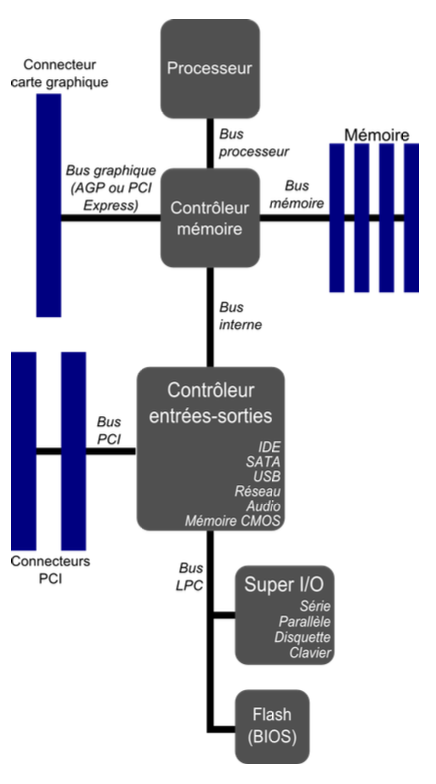
\includegraphics[width=0.2\textwidth]{Images/View/view.png}
    \caption{View}
    \label{fig:myimage}
  \end{figure}
  

\subsection{Processeur}


Le \textbf{processeur} exécute les instructions et réalise les traitements. 
Il est caractérisé par son jeu d'instructions (Instruction Set Architecture), qui définit les instructions exécutables et leur format d'encodage (opcode et opérandes). 
Les instructions sont classées en plusieurs types :
\begin{itemize}
    \item Arithmétique (e.g. \texttt{add}, \texttt{div})
    \item Logique (e.g. \texttt{and})
    \item Accès mémoire (e.g. \texttt{lw}, \texttt{sw})
    \item Instructions système
\end{itemize}

Les processeurs modernes utilisent une structure de pipeline, permettant à différentes instructions d'occuper simultanément différentes parties du pipeline. 
Deux types principaux d'architecture de jeu d'instructions existent :
\begin{itemize}
    \item RISC (Reduced Instruction Set Computer)
    \item CISC (Complex Instruction Set Computer)
\end{itemize}

Les responsabilités de gestion du processeur en collaboration avec le système d'exploitation incluent :
\begin{itemize}
    \item Surveillance de l'exécution des instructions
    \item Répartition du temps processeur entre différents programmes
\end{itemize}


\subsubsection{Exécution de programme}

La première responsabilité de gestion consiste à surveiller l'exécution des instructions d'un programme utilisant le processeur. 
Le système d'exploitation et les programmes se partagent le processeur, nécessitant la suspension de l'exécution en cours lors d'un évènement particulier. 
Le processeur peut réagir de différentes manières :

\begin{itemize}
    \item \textbf{Mauvais comportement} : déroutement vers une fonction du système d'exploitation pour traiter des erreurs telles qu'une division par zéro, un accès mémoire invalide ou une tentative d'exécuter une instruction privilégiée.
    \item \textbf{Anomalie non fatale} : correction des circonstances ayant provoqué l'anomalie et reprise de l'exécution.
    \item \textbf{Appel système} : branchement vers une fonction du système d'exploitation pour des demandes comme l'obtention de mémoire ou l'écriture dans un fichier.
    \item \textbf{Interruption externe} : traitement d'une interruption provenant d'un périphérique externe. 
    Par exemple, une interruption du clavier nécessite de communiquer avec le contrôleur du clavier pour identifier la touche concernée et le programme destinataire.
\end{itemize}


\subsubsection{Ordonnancement de programmes}

La seconde responsabilité du système d'exploitation est de répartir le temps processeur entre les programmes. 
L'ordonnancement sélectionne le prochain programme à exécuter lorsque le processeur est libre. 
Différentes stratégies sont utilisées selon le type de système et la charge de travail. 
Les métriques d'évaluation incluent la minimisation du temps d'exécution moyen et l'adéquation entre les besoins du programme et le temps processeur alloué.


\subsection{Mémoire}

La mémoire stocke les données de travail des programmes et est organisée en une hiérarchie :
\begin{itemize}
    \item \textbf{Caches} (e.g. L1, L2) : Intermédiaires entre les registres et la mémoire principale, stockant temporairement les données fréquemment accédées (principe de localité).
    \item \textbf{Mémoire principale} (e.g. RAM, GPU) : Stocke les données de travail (e.g. tableaux, variables, stack) lorsqu'il n'y a pas de registres disponibles.
    \item \textbf{Mémoire secondaire} (e.g. HDD, SSD) : Utilisée comme espace temporaire (swap) lorsque la mémoire principale est pleine.
\end{itemize}

L'allocation dynamique permet de gérer la mémoire de manière flexible. La mémoire virtuelle charge/décharge les données non actives pour pallier les limitations de la mémoire physique (e.g. adressage 32 bits, 0x00000000 à 0xffffffff).


\subsubsection{Protection de la mémoire}

Le système d'exploitation contrôle les accès mémoire pour garantir qu'un programme n'accède qu'à sa propre mémoire, évitant ainsi la lecture ou la modification de données sensibles (e.g. clefs de chiffrement). 
Le processeur vérifie les accès mémoire selon les descriptions des espaces mémoire accessibles à chaque programme, mises à jour par le système d'exploitation.

\begin{itemize}
    \item \textbf{Adresse valide} : Accessible au programme, l'accès est accordé (e.g. \texttt{lw}, \texttt{sw}).
    \item \textbf{Adresse indisponible} : Accessible mais non présente en mémoire principale, nécessite un chargement depuis la mémoire secondaire.
    \item \textbf{Adresse invalide} : Hors de l'espace accessible, entraîne l'arrêt du programme.
\end{itemize}



\subsubsection{Répartition de la mémoire}

La seconde responsabilité de gestion est la répartition de la mémoire principale entre les différents programmes. 
Cela inclut la représentation et le suivi des portions de mémoire (libres ou non) et l'identification d'une portion adéquate pour satisfaire une demande d'allocation dynamique.

\subsection{Stockage}

Le stockage préserve les données produites par un programme au-delà de son exécution. Une fois le programme terminé, sa mémoire est libérée et peut être allouée à un autre programme. 
La notion de fichier assure la pérennité des données, malgré la diversité des supports physiques adaptés à différents scénarios d’utilisation :

\begin{itemize}
    \item \textbf{HDD} : Disque dur, bon marché, accès lent, organisé en plateaux, cylindres, têtes, et secteurs.
    \item \textbf{SSD} : Disque à état solide, rapide, coût plus élevé, organisé en blocs et pages.
    \item \textbf{Bande magnétique} : Grande capacité, fiable, utilisé pour les backups.
\end{itemize}

Un système de fichiers met en place une abstraction pour accéder au stockage, en représentant les fichiers et répertoires et leurs méta-données (e.g. taille, dates, permissions). 
Il garantit également la cohérence des écritures et réduit la possibilité de corruption des données.

\subsection{Typologie des systèmes}

Les types de systèmes influencent la conception des systèmes d'exploitation :

\begin{itemize}
    \item \textbf{Mainframe} : Exécute des jobs réguliers avec des E/S intensives (e.g. calcul des fiches de paie). 
    Supporte un grand volume de transferts et offre une gestion de timesharing pour plusieurs utilisateurs.
    \item \textbf{Serveur} : Fournit des services aux utilisateurs distants (e.g. serveur d'impression), gère les ressources et la facturation.
    \item \textbf{Personal Computer} : Interaction humaine via interface graphique, exécution simultanée de plusieurs programmes, interactivité centrale (mesurée par la latence entre l'action et la réaction).
    \item \textbf{Système mobile} (e.g. tablette, smartphone) : Contraintes de ressources, économie d'énergie cruciale, processeur et mémoire limités, alimentation par batterie.
    \item \textbf{Système embarqué} (e.g. TV, voiture) : Logiciel prédéterminé pour une machine spécifique, pas de flexibilité pour l'installation d'applications supplémentaires.
    \item \textbf{Système de senseurs} : Surveille des paramètres environnementaux (e.g. température, humidité), transmet les données à un central, optimisé pour faible consommation d'énergie.
    \item \textbf{Système temps-réel} : Respect des échéances crucial, priorisation des tâches, gestion précise du temps pour aligner les traitements avec l'environnement.
\end{itemize}

\subsection{Architecture}

Un système d'exploitation inclut le code, les données, et la stack, similaires à un programme classique. Il utilise des instructions système nécessitant des niveaux de privilège spécifiques, et le noyau gère les ressources.

\begin{itemize}
    \item \textbf{Noyau monolithique} : Code dans un fichier unique, exécuté au plus haut niveau de privilège. Exemple : système avec configuration matérielle fixe.
    \item \textbf{Noyau modulaire} : Base toujours en mémoire, modules chargés/déchargés selon les besoins. Exemple : Linux.
    \item \textbf{Microkernel} : Composantes exécutées à des niveaux de privilège réduits pour éviter les compromissions. 
    Un serveur de ré-incarnation gère les erreurs fatales. Exemple : MINIX3.
    \item \textbf{Exokernel} : Gestion des ressources laissée aux programmes, le noyau assure uniquement la protection et l'isolation. Exemple : machines virtuelles.
\end{itemize}


\subsection{Rôles et fonctions du système d'exploitation}
Les principales fonctions d'un SE incluent :
\begin{itemize}
    \item \textbf{Gestion des processus} : Supervise la création, l'exécution, la suspension et la terminaison des processus. 
    Il gère également les threads et les mécanismes de synchronisation.
    \item \textbf{Gestion de la mémoire} : Alloue et libère de la mémoire, gère la mémoire virtuelle, et s'assure que chaque processus a un espace mémoire isolé et protégé.
    \item \textbf{Gestion des entrées/sorties (I/O)} : Coordonne et contrôle les opérations d'entrée/sortie des périphériques, utilisant des pilotes pour assurer la communication entre le matériel et les logiciels.
    \item \textbf{Gestion des fichiers} : Gère les fichiers sur les différents systèmes de stockage, offrant des opérations de lecture, écriture, création, et suppression de fichiers.
    \item \textbf{Sécurité et protection} : Protège les données et les ressources contre les accès non autorisés et les défaillances, assurant l'intégrité et la confidentialité des informations.
\end{itemize}


\subsection{Défis de la conception des systèmes d'exploitation}
La conception d'un SE implique de nombreux défis, notamment :
\begin{itemize}
    \item \textbf{Complexité du matériel} : La gestion de divers composants matériels nécessite des abstractions et des interfaces standardisées.
    \item \textbf{Multiplicité des utilisateurs et des tâches} : Assurer une utilisation équitable et efficace des ressources tout en isolant les utilisateurs et les tâches pour éviter les interférences.
    \item \textbf{Sécurité et fiabilité} : Protéger le système contre les attaques et les défaillances tout en maintenant une performance stable.
    \item \textbf{Évolutivité} : Adapter le SE aux nouveaux matériels et aux besoins croissants des utilisateurs sans compromettre les performances.
\end{itemize}

\subsection{Conclusion}
Les systèmes d'exploitation sont des composants essentiels des systèmes informatiques, assurant la gestion et la coordination des ressources matérielles et logicielles. 
Une compréhension approfondie de leurs fonctions, types et défis est cruciale pour les étudiants en sciences informatiques, permettant de développer des applications efficaces et sécurisées.


\newpage
\section{Description}\label{sec:description}

L'anonymat en ligne, objet de ce rapport au travers de l'analyse de \acrshort{tor}, va de pair avec une latence accrue en raison des différentes techniques et méthodes mises en place pour y parvenir.
Si \acrshort{tor} et le routage oignon sur lequel il repose font partie des systèmes dits de faible latence, les premiers à offrir l'anonymat appartenaient à une seconde catégorie dite à forte latence.

\textbf{Prémices de l'anonymat (0G)}

En 1981, Chaum introduisit la notion de mixnets (réseaux mélangés) \cite{chaum_cmix_nodate} afin de permettre aux utilisateurs d'utiliser un réseau sans compromettre leur anonymat.
Il était alors question de redéfinir l'ordre dans lequel les messages étaient transmis à travers le réseau: un message pouvait arriver en premier dans un noeud, mais être transmis après les 3 messages suivants.
Ce système permettait d'empêcher le suivi des données entre noeuds.
Si l'anonymat était garanti, des taux de latence particulièrement élevés venaient restreindre son utilité pour des usages nécessitant des temps de réponses réduits.
En effet, les mixnets étants basés uniquement sur la \acrfull{ac}, ils ne sont pas adaptés à des usages interactifs.

\textbf{Routage en Oignon (1G)}

Initialement développé dans les années 1990, le routage en oignon est venu résoudre ces problèmes en anonymisant des applications basées sur TCP, telles que la navigation web et la messagerie instantanée et les connexions SSH avec un taux de latence réduit.
Ce système, bien que novateur, présentait plusieurs lacunes significatives, notamment l'absence de sécurité parfaite vers l'avant, qui signifie que la sécurité des données n'était pas garantie si une partie du chemin était compromise après la transmission des données. 
De plus, il nécessitait des proxies d'application distincts pour chaque protocole de la 7e couche du modèle OSI supporté (\textit{e.g.,} HTTPS, FTP,\dots).
Ce qui a limité sa polyvalence ainsi que son efficacité face à divers types de traffics en ajoutant des couches de traitements supplémentaires.


% \textbf{Alternatives}

% \begin{table}[htbp]
    \centering
    \begin{tabularx}{\textwidth}{
        >{\raggedright\arraybackslash}p{2cm} 
        >{\raggedright\arraybackslash}X}
    \toprule
    \rowcolor[HTML]{EFEFEF}
    \textbf{Travail} & \textbf{Description} \\
    \midrule
    Chaum's Mix-Net & Chaum a proposé de cacher la correspondance entre l'expéditeur et le destinataire en enveloppant les messages dans des couches de cryptographie à clé publique et en les relayant à travers un chemin composé de "mélanges". Chaque mélange décrypte, retarde et réordonne les messages avant de les relayer. \\
    \midrule
    Babel, Mixmaster, Mixminion & Ces systèmes cherchent à maximiser l'anonymat au coût d'introduire des latences comparativement grandes et variables. Ils résistent aux adversaires globaux forts mais introduisent trop de décalage pour des tâches interactives comme la navigation web, le chat Internet ou les connexions SSH. \\
    \midrule
    \acrshort{tor} & \acrshort{tor} appartient à la catégorie des conceptions à faible latence qui tentent d'anonymiser le trafic réseau interactif. Ces systèmes gèrent une variété de protocoles bidirectionnels et fournissent une livraison de courrier plus pratique que les réseaux de courrier électronique anonymes à haute latence. Toutefois, ils peinent à empêcher un attaquant capable d'écouter les deux extrémités de la communication de corréler le timing et le volume du trafic entrant et sortant du réseau d'anonymat. \\
    \midrule
    Anonymizer (Single-hop proxies) & Ces conceptions utilisent un serveur unique de confiance pour supprimer l'origine des données avant de les relayer. Ces conceptions sont faciles à analyser mais les utilisateurs doivent faire confiance au proxy anonymisant. Concentrer le trafic en ce point unique augmente le jeu d'anonymat, mais cela devient vulnérable si l'adversaire peut observer tout le trafic entrant et sortant du proxy. \\
    \midrule
    Java Anon Proxy (JAP \acrshort{or} Web MIXes) & Utilise des routes partagées fixes appelées cascades. Comme avec un proxy à un seul saut, cette approche agrège les utilisateurs en ensembles d'anonymat plus larges, mais un attaquant n'a besoin d'observer que les deux extrémités de la cascade pour relier tout le trafic du système. \\
    \midrule
    PipeNet & Un autre design à faible latence, offrant une meilleure anonymat mais permettant à un seul utilisateur d'arrêter le réseau en ne transmettant pas de données. \\
    \midrule
    Tarzan, MorphMix, Crowds & Ces systèmes P2P tentent de dissimuler si un pair donné a initié une demande ou simplement relayé celle-ci. Tarzan et MorphMix utilisent le chiffrement par couches, tandis que Crowds suppose qu'un adversaire ne peut pas observer l'initiateur. Hordes, basé sur Crowds, utilise des réponses multicast pour masquer l'initiateur. \\
    \midrule
    Freedom, original Onion Routing & Construisent des circuits d'un seul coup en utilisant des couches de messages chiffrés avec des clés publiques. Tor, Tarzan, MorphMix, Cebolla, et le réseau d'anonymat de Rennhard construisent des circuits par étapes, en les étendant un saut à la fois. \\
    \bottomrule
    \end{tabularx}
    \caption{Systèmes d'anonymat}
    \label{tab:systems}
    \end{table}
    
% \begin{table}[htbp]
    \centering
    \begin{tabularx}{\textwidth}{
        >{\raggedright\arraybackslash}X
        >{\raggedright\arraybackslash}X
        >{\raggedright\arraybackslash}X
        >{\raggedright\arraybackslash}X
        >{\raggedright\arraybackslash}X}
        \toprule
    \rowcolor[HTML]{EFEFEF}    
    \textbf{Système} & \textbf{Latence} & \textbf{Anonymat} & \textbf{Utilisation principale} & \textbf{Vulnérabilités} \\
    \midrule
    Chaum's Mix-Net & Haute & Très élevé & Messages asynchrones & Délais et réordonnancement \\
    \midrule
    Mixmaster & Haute & Très élevé & Email anonyme & Latence élevée, peu interactif \\
    \midrule
    Mixminion & Haute & Très élevé & Email anonyme & Latence élevée, peu interactif \\
    \midrule
    \acrshort{tor} & Faible & Élevé & Trafic interactif (Web, SSH) & Corrélation de timing et de volume \\
    \midrule
    Anonymizer & Très faible & Faible & Proxy unique, navigation Web & Confiance en un seul point, vulnérable à l'observation globale \\
    \midrule
    Java Anon Proxy (JAP) & Faible & Élevé & Web MIXes, routes fixes & Observation des extrémités de cascade \\
    \midrule
    PipeNet & Faible & Très élevé & Réseau à faible latence & Réseau arrêté par utilisateur unique \\
    \midrule
    Tarzan & Faible & Élevé & Réseau P2P & Complexité, difficulté de déploiement \\
    \midrule
    MorphMix & Faible & Élevé & Réseau P2P & Complexité, difficulté de déploiement \\
    \midrule
    Crowds & Faible & Moyen & Anonymat pour requêtes HTTP & Pas de chiffrement à clé publique \\
    \midrule
    Hordes & Faible & Moyen & Basé sur Crowds, réponses multicast & Latence, complexité accrue \\
    \midrule
    Freedom & Faible & Élevé & Réseau d'oignons original & Complexité, nécessités de patchs kernel \\
    \bottomrule
    \end{tabularx}
    \caption{Comparaison des systèmes d'anonymat}
    \label{tab:systems-vs}
    \end{table}
    

\textbf{Evolution vers \acrshort{tor} (2G)}

En réponse à ces défis, \acrfull{tor} a été introduit en 2002, marquant une évolution majeure du concept original. 

\begin{quote}
    \textit{Onion Routing is a distributed overlay network designed to anonymize TCP-based applications like web browsing, secure shell, and instant messaging.} \cite[p.~1, sec.~1]{dingledine_tor_2004}
\end{quote}

Il est important de noter que le protocole \acrshort{udp} n'est actuellement pas pris en charge par \acrshort{tor}.
En effet, ce dernier ne nécessitant pas de connexion et donc d'accusé de réception, cela le rend intrinsèquement plus complexe à anonymiser sans induire une latence importante qui serait contraire aux objectifs de conception du réseau.

\acrshort{tor} a introduit plusieurs améliorations significatives :
\begin{itemize}
    \item Sécurité parfaite vers l'avant : Cette fonctionnalité assure que, même si un nœud intermédiaire est compromis, les données transmises antérieurement restent protégées.
    \item Simplification des proxies d'application : Grâce à l'adoption de l'interface proxy standard SOCKS, \acrshort{tor} supporte plusieurs types de trafic \acrshort{tcp} sans nécessiter de modifications logicielles spécifiques, augmentant ainsi sa flexibilité et réduisant la complexité technique.
    \item Contrôle de congestion décentralisé : \acrshort{tor} améliore la réactivité du système et la gestion de la charge réseau par un mécanisme de contrôle de congestion qui ne nécessite pas de communication inter-nœuds, facilitant ainsi une meilleure scalabilité et performance du réseau.
\end{itemize}


Les utilisateurs établissent des circuits sécurisés à travers le réseau, où chaque nœud, ou "routeur oignon", ne connaît que le nœud précédent et le suivant. Les données transitent en cellules chiffrées, chaque nœud dévoilant progressivement le chemin jusqu'à la destination finale, ce qui préserve l'anonymat de la source et de la destination.

\textbf{Défis et Perspectives (3G)}

Malgré ses avancées, \acrshort{tor} fait face à des défis continus, notamment en matière de latence réseau et de résistance aux attaques d'analyse de trafic, où des adversaires sophistiqués pourraient théoriquement corréler les modèles de trafic entrant et sortant pour compromettre l'anonymat. Les efforts continus de la communauté pour mettre à jour et améliorer \acrshort{tor} sont cruciaux pour répondre aux défis de l'Internet moderne et maintenir la robustesse du système face aux menaces émergentes.

En résumé, \acrshort{tor} représente une solution robuste et flexible pour l'anonymat en ligne, mais comme tout système, il n'est pas exempt de limitations qui doivent être adressées pour assurer son efficacité à long terme.
La Section \ref{sec:v3} "\nameref{sec:v3}" concerne la 3e génération du routage oignon.

\newpage
\section{Conception}\label{sec:design}
La communication dans \acrshort{tor} se fait au travers de flux de données composés de cellules et empruntant des circuits prédéfinis.

\begin{enumerate}
    \item \ref{subsec:cellule} \nameref{subsec:cellule} de types contrôle ou relais, leurs fonctions sont spécifiques.
    \item \ref{subsec:circuit} \nameref{subsec:circuit} construits via des cellules de contrôles, ils transmettent les données via des cellules de relais.
\end{enumerate}
\subsection{Cellules}\label{subsec:cellule}

D'une taille fixe de 512 octets, elles se divisent en deux parties principales : un en-tête (header) et une charge utile (payload). 
L'en-tête contient un identifiant de circuit (circID) et une commande (CMD), comme illustré ci-dessous dans le schéma de la Figure \ref{fig:structure-cellule}.

\begin{figure}[h!]
    \centering
    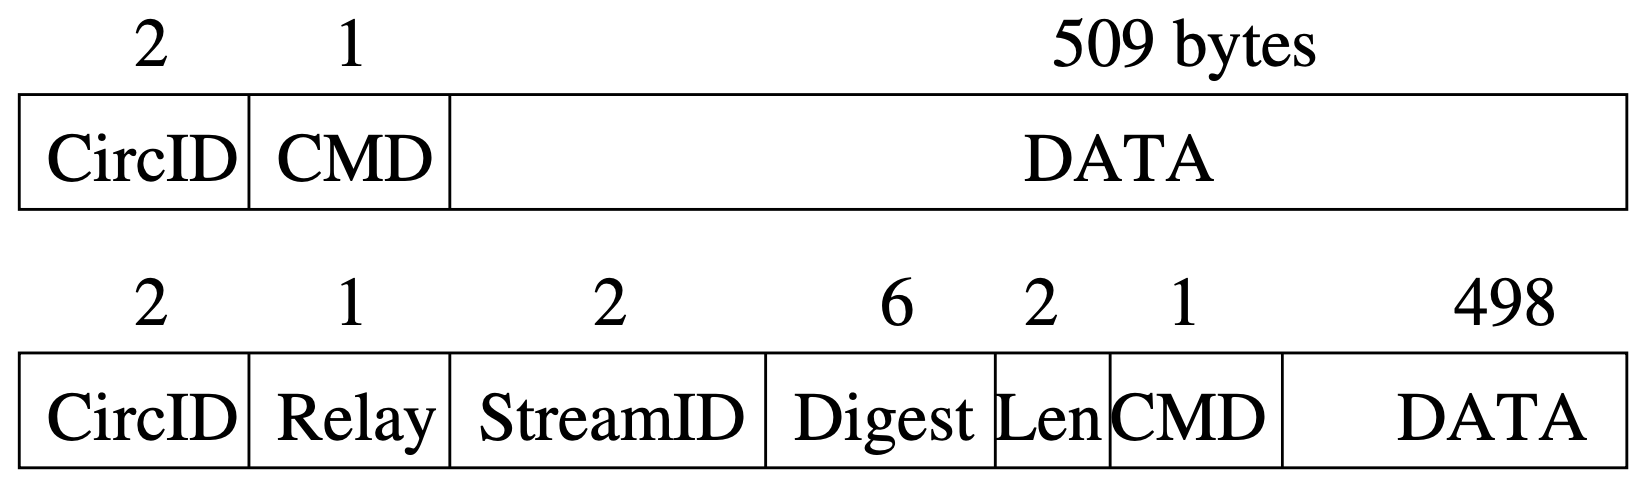
\includegraphics[width=0.5\linewidth]{Images/Diagrams/cellule.png}
    \caption{Structure de cellule vs structure d'une cellule de relais. \cite[Tor: The Second-Generation Onion Router]{dingledine_tor_2004}}
    \label{fig:structure-cellule}
\end{figure}

Il existe deux types de cellules distincts:
\begin{enumerate}
    \item Contrôle : les cellules de contôle sont traitées directement par le noeud qui les reçoit; leurs fonctions sont administratives: initialisation, maintenance et clôture du circuit.
    \item Relais : les cellules de relais permettent le transfert de bout en bout des données utilisateur, leurs fonctions concernent le flux de données
\end{enumerate}

Le tableau \ref{tab:cellules-tor} "\nameref{tab:cellules-tor}" ci-dessous reprend l'ensemble des différents types de cellules utilisées dans \acrshort{tor}.
Les commandes y sont spécifiques aux type dont il est question.

\begin{table}[htbp]
    \centering
    \begin{tabularx}{\textwidth}{
        >{\raggedright\arraybackslash}p{2cm} 
        >{\raggedright\arraybackslash}X 
        >{\raggedright\arraybackslash}X}
            \toprule
            \rowcolor[HTML]{EFEFEF}
            \textbf{Type}           & \textbf{Commandes}        & \textbf{Fonctions} \\
            \midrule
            Contrôle & PADDING & Garder la connexion active \\
            & CREATE & Établir un nouveau circuit \\
            & CREATED & Confirmer la création du circuit \\
            & DESTROY & Fermer un circuit \\
            \addlinespace
            Relais & RELAY\_BEGIN & démarrer une connexion \acrshort{tcp} \\
            & RELAY\_DATA & transfert de données \\
            & RELAY\_END & fermer une connexion \acrshort{tcp} \\
            & RELAY\_CONNECTED & confirmer l'établissement de la connexion \acrshort{tcp} \\
            & RELAY\_EXTEND & étendre un circuit à un autre nœud \\
            & RELAY\_TRUNCATED & signaler une coupure de circuit partielle \\
            & RELAY\_SENDME & contrôle de congestion (demande de données) \\
            \bottomrule
    \end{tabularx}
    \caption{Comparaison des Types de Cellules et de leurs commandes dans le Réseau Tor}
    \label{tab:cellules-tor}
\end{table}

\newpage
\subsection{Circuits}\label{subsec:circuit}

Contrairement à la première génération de routage onion, chaque circuit peut multiplexer différents flux TCP.
Ces circuits sont reconstruits chaque minute par les \acrshort{op} afin de limiter les liens entre flux (rotation périodique).

Les circuits sont composés de trois types de n\oe uds:
\begin{itemize}
    \item Gardien d'entrée
    \item Noeud(s) intermédiaire(s)
    \item Noeud de sortie
\end{itemize}


Sur la Figure \ref{fig:flowdiagram} "\nameref{fig:flowdiagram}" ci-dessous, "\acrshort{or} 1" représente le "Gardien d'entrée" tandis que "\acrshort{or} 2" représente le "Noeud de sortie".
Le processus est initié par l'expéditeur, qui utilise des cellules de contrôle afin de construire le circuit.
Lorsque la connection avec le premier  \acrshort{or}  est établie via une cellule de création, le processus continue jusqu'à atteindre la destination finale.
Une fois le circuit construit, des cellules de relais le parcourent jusqu'à atteindre la destination et retourner le résultat à l'expéditeur.

\begin{figure}[h!]
    \centering
    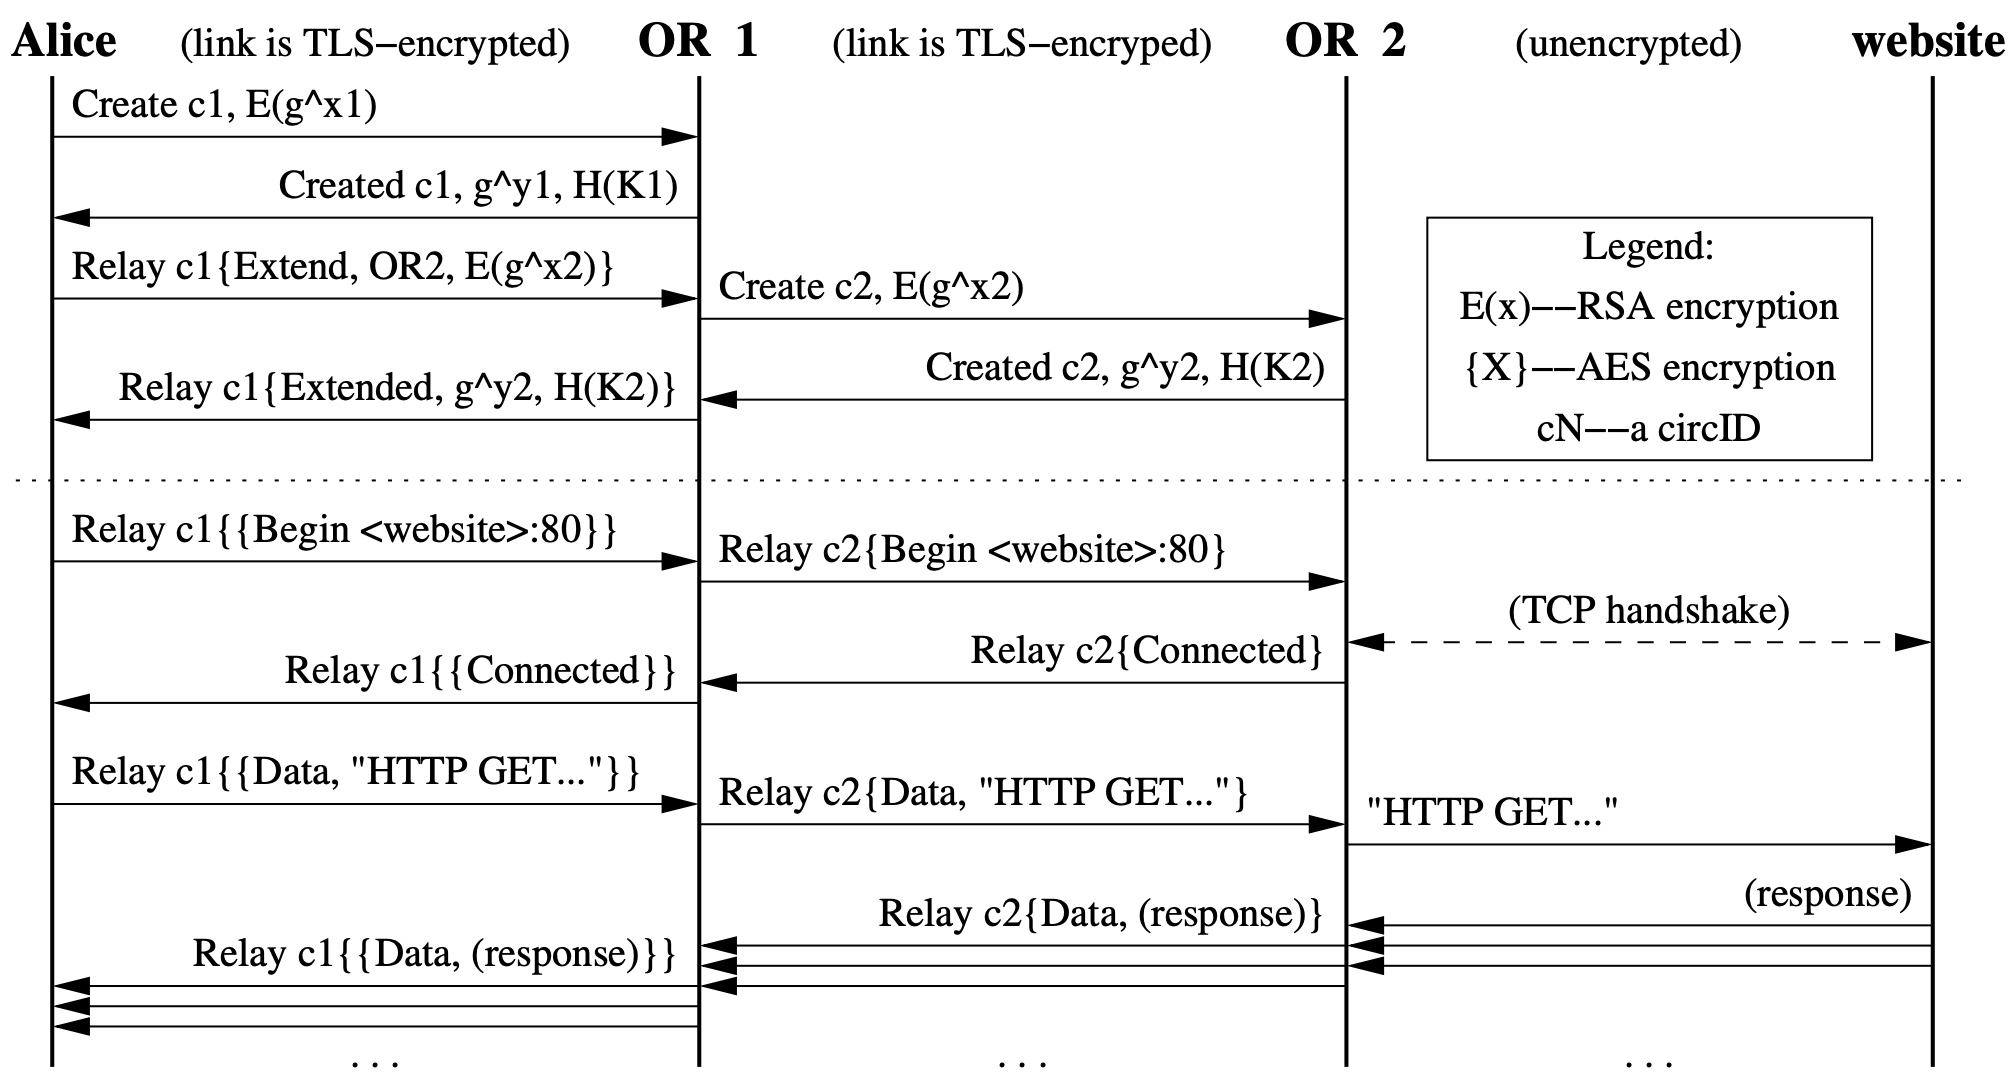
\includegraphics[width=\linewidth]{Images/Diagrams/flow.png}
    \caption{Circuit à deux Routeurs Onions permettant à Alice de joindre un site web.\cite[Tor: The Second-Generation Onion Router]{dingledine_tor_2004}}
    \label{fig:flowdiagram}
\end{figure}


\newpage
\section{S\'ecurit\'e}\label{sec:security}

La sécurité au sein de \acrshort{tor} s'articule autour d'un réseau de noeuds relais comprenant un noeud d'entrée, des noeuds intermédiaires ainsi qu'un noeud de sortie.
Lors de l'initialisation de la connexion entre l'expéditeur et le destinataire, des méthodes cryptographiques avancées (\textit{cfr.}, sec. \ref{subsec:data} "\nameref{subsec:data}") sont utilisées afin de sécuriser non seulement les données transmises mais également leurs canaux de communications.
Le routage en oignon offre l'anonymat en encapsulant les données dans plusieurs couches de chiffrement. 
Chaque nœud dans le circuit ne peut déchiffrer que la couche lui étant assignée, ne révélant jamais l'identité ni de l'expéditeur ni du destinataire.

Les aspects techniques de la sécurité dans \acrshort{tor}, incluant le routage en oignon, la sélection des relais, les protocoles de chiffrement, les mesures défensives et les politiques de confidentialité, contribuent à sa robustesse comme outil d'anonymat en ligne.

La sécurité dans \acrshort{tor} passe par le chiffrement des données ainsi que par la sécurisation des communications.
\begin{enumerate}
  \item \ref{subsec:data} \nameref{subsec:data} chiffrées via cryptographie symétrique et asymétrique
  \item \ref{subsec:comm} \nameref{subsec:comm} sécurisées via poignées de mains \acrfull{dh} et \acrfull{tls}
\end{enumerate}

La Figure \ref{fig:structure-layers} "\nameref{fig:structure-layers}" ci-dessous illustre les différentes couches de sécurité qui se supperposent dans \acrshort{tor}.
Les données étant transmises via des cellules chiffrées via cryptographie symétrique. 
La cryptographie symétrique (\acrshort{sc}) découle d'un processus impliquant la cryptographie asymétrique (\acrshort{ac}) elle-même impliquant les poignées de mains Diffie-Hellman (\acrshort{dh}).
Il est important de noter que les poignées de main \acrshort{dh} ainsi que la \acrshort{ac} n'interviennent qu'au moment de l'établissement du circuit.
Ces dernières utilisent des canaux de communications sécurisés via le protocole \acrshort{tls}.


\begin{figure}[htbp]
  \centering
  \begin{tikzpicture}
    % Main figure
    \node[inner sep=0] (main) {
      \begin{tikzpicture}
        % Layers with hatching
        \begin{scope}
            \clip (0,0) circle (2.2cm);
            \fill[pattern=north west lines] (0,0) circle (2.2cm);
            \fill[white] (0,0) circle (1.3cm);
        \end{scope}
        % Circles and labels
        \draw (0,0) circle (0.7cm) node[align=center] {Cell};
        \draw (0,0) circle (1.3cm) node[yshift=1cm] {SC};
        \draw (0,0) circle (2.2cm) node[yshift=1.7cm] {DH \&\& AC};
        \draw (0,0) circle (2.8cm) node[yshift=2.5cm] {TLS};
      \end{tikzpicture}
    };

    % Legend
    \node[right=10mm of main, inner sep=10pt, draw, rectangle, minimum width=3cm, minimum height=2.5cm, text width=2.8cm] (legend) {
      \raggedright
      \tikz{\fill[pattern=north west lines, pattern color=black] (0,0) rectangle (0.5,0.5);} Initialisation only\\[1ex]
      \tikz{\draw (0,0.25) circle (0.25);} Permanent layers
    };

  \end{tikzpicture}
  \caption{Modélisation des différentes couches de sécurité dans TOR}
  \label{fig:structure-layers}
\end{figure}



\newpage
\subsection{Données}\label{subsec:data}

La sécurité au niveau des données est assurée par une combinaison de cryptographie asymétrique et symétrique pour sécuriser le contenu.

\begin{enumerate}
  \item \ref{subsubsec:cs} \nameref{subsubsec:cs} Utilisée pour déchiffrer les cellules de données transmises.
  \item \ref{subsubsec:ca} \nameref{subsubsec:ca} Utilisée pour l'échange de clés privées.
\end{enumerate}


\subsubsection{Cryptographie symétrique}\label{subsubsec:cs}

La cryptographie symétrique repose sur l'utilisation de clés privées partagées.
Le protocole d'échange de clés \acrlong{dh} permet d'établir la connexion et de générer les clés privées via l'algorithme AES (Advanced Encryption Standard).
Ces clés peuvent être comparées à un cadenas: un code protège le cadenas, quiconque possède le code peut ouvrir ce cadenas, cependant si le code venait à être partagé, cela compromettrait la sécurité apportée par ce cadenas.

La Figure \ref{fig:structure-chiffrement} "\nameref{fig:structure-chiffrement}" ci-dessous illustre la structure de chiffrement d'une cellule au sein du réseau \acrshort{tor}.
La première couche de chiffrement sera déchiffrée par le premier noeud du circuit. 
L'oignon sera ainsi épluché jusqu'à atteindre le dernier noeud et retirer sa dernière couche.
Ce processus permettra ainsi au message d'être transmis au destinataire de manière sécurisée.

\begin{figure}[h!]
  \centering
  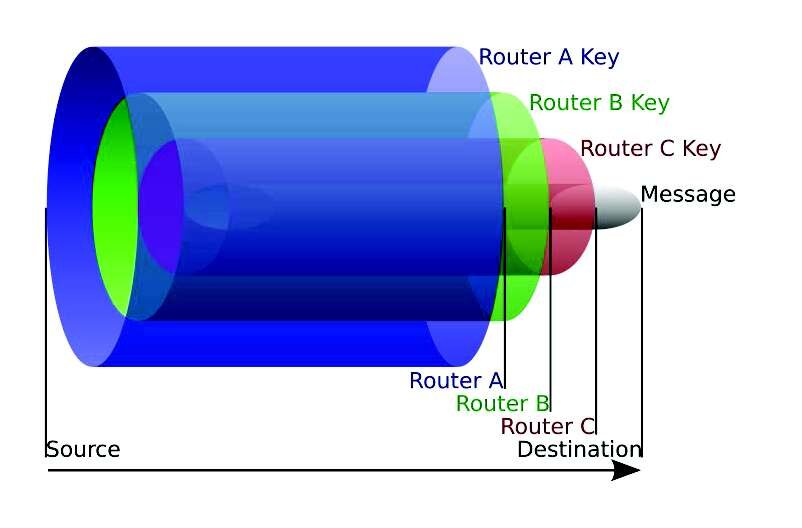
\includegraphics[width=0.7\linewidth]{Images/OR/Layers-of-the-Onion-source.png.jpeg}
  \caption{Structure du chiffrement en couches. \cite[Layers-of-the-Onion-source]{noauthor_layers---onion-sourcepng_nodate}.}
  \label{fig:structure-chiffrement}
\end{figure}

\subsubsection{Cryptographie asymétrique}\label{subsubsec:ca}

La cryptographie asymétrique repose sur l'utilisation d'une paire de clés publique et privée associées.
Ces clés sont mathématiquement liées: dans \acrshort{rsa} il s'agit de la factorisation de grands nombres premiers tandis que dans \acrshort{ecc} il s'agit de logarithmes discrets.

Un message chiffré avec une clé publique ne peut être déchiffré qu'avec la clé privée correspondante: si une personne reçoit un message lui demandant de crier dans un auditoire afin de pouvoir la situer, lorsque celle-ci criera, seule la personne qui le lui aura demandé sera en mesure de déchiffrer le message "Je suis ici", les autres ne disposant tout simplement pas des clés permettant de décoder la situation.
Dans cet exemple, la clé publique est le système de messagerie permettant de cacher le contenu du message aux autres personnes présentes. La clé privée est le contenu du message en lui-même.

\subsubsection{Comparaison cryptographie symétrique et asymétrique}

Le Tableau \ref{tab:tech-crypto} "\nameref{tab:tech-crypto}" ci-dessous permet de mettre en évidence les différences d'usages entre cryptographie symétrique et asymétrique.
D'un côté une cryptographie plus simple à mettre en place et plus adaptée pour le transfert d'importants volumes de données.
De l'autre une cryptographie plus exigeante mais offrant d'avantages de garanties lors du partage de données particulièrement sensibles.
% \begin{table}[htbp]
%     \centering
%     \begin{tabularx}{\textwidth}{
%         >{\raggedright\arraybackslash}p{2cm} 
%         >{\raggedright\arraybackslash}p{6.5cm} 
%         >{\raggedright\arraybackslash}p{6.5cm}}
%         \toprule
%         \rowcolor[HTML]{EFEFEF}
%         \textbf{}               & \textbf{Clés Symétriques}                                                                                                                         & \textbf{Clés Asymétriques} \\
%         \midrule
%         Méthode de chiffrement  & Utilise la même clé pour le chiffrement et le déchiffrement, ce qui rend le processus plus direct mais nécessite une gestion sécurisée de la clé. & Utilise une paire de clés: une publique pour le chiffrement et une privée pour le déchiffrement, facilitant la distribution des clés mais augmentant la complexité. \\
%         \midrule
%         Vitesse                 & Plus rapide due à des opérations moins complexes, idéale pour le chiffrement de grands volumes de données.                                        & Plus lent à cause des opérations cryptographiques plus complexes, adapté pour le chiffrement d'informations sensibles en petites quantités. \\
%         \midrule
%         Gestion des clés        & Nécessite une méthode sécurisée pour partager la clé entre les parties, moins adapté pour les systèmes à grande échelle.                          & La gestion des clés est simplifiée puisque la clé publique peut être distribuée ouvertement, tandis que la clé privée reste secrète. \\
%         \midrule
%         Usage typique           & Favorisé pour le chiffrement des données en transit, comme dans le cas des cellules Tor, où la performance et l'efficacité sont cruciales.        & Utilisé pour les échanges sécurisés initiaux, tels que l'établissement de clés symétriques ou la vérification d'identité, grâce à la sécurité renforcée qu'il offre. \\
%         \bottomrule
%     \end{tabularx}
%     \caption{Comparaison entre clés symétriques et asymétriques}
%     \label{tab:cles-sym-asym}
% \end{table}


% \begin{table}[htbp]
%     \centering
%     \begin{tabularx}{\textwidth}{
%         >{\raggedright\arraybackslash}p{2cm}
%         >{\raggedright\arraybackslash}X
%         >{\raggedright\arraybackslash}X}
%         \toprule
%         \rowcolor[HTML]{EFEFEF}
%         \textbf{}                   & \textbf{Cryptographie Symétrique} & \textbf{Cryptographie Asymétrique} \\
%         \midrule
%         Méthode de chiffrement      & Utilise une seule clé pour chiffrer et déchiffrer les données. & Utilise une paire de clés: une publique pour chiffrer, une privée pour déchiffrer. \\
%         \midrule
%         Algorithmes                 & AES et DES &  \acrshort{rsa} et \acrshort{ecc} \\
%         \midrule
%         Complexité algorithmique    & Opérations basées principalement sur des transformations linéaires simples (par exemple, permutation et substitution). Moins coûteux en termes de ressources de calcul. & Nécessite des opérations mathématiques complexes telles que l'exponentiation modulaire, ce qui entraîne des temps de traitement plus longs et une consommation plus élevée de ressources. \\
%         \midrule
%         Gestion des clés            & La distribution sécurisée des clés pose un défi majeur car chaque paire d'utilisateurs nécessite une clé unique partagée, escaladant le nombre de clés nécessaire de manière exponentielle avec le nombre d'utilisateurs. & Facilite la distribution des clés; seule la clé publique doit être partagée ouvertement, tandis que la clé privée est gardée secrète par chaque utilisateur, simplifiant la gestion des clés même dans de grands réseaux. \\
%         \midrule
%         Utilisation                 & Idéal pour les environnements où la sécurité des lignes de communication des clés peut être garantie. Couramment utilisé pour le chiffrement de données au repos et le chiffrement de masse de données en transit. & Utilisé principalement pour les transactions sécurisées, l'authentification et les signatures numériques où les clés ne doivent pas être échangées via un canal sécurisé, réduisant ainsi le risque d'exposition des clés. \\
%         \midrule
%         Vulnérabilités typiques     & Susceptible à l'analyse des clés si des clés insuffisamment aléatoires ou courtes sont utilisées, ou si la gestion des clés est compromise. & Plus vulnérable aux attaques cryptanalytiques telles que l'attaque par facteurisation pour \acrshort{rsa} ou les attaques sur la logique elliptique pour ECC, en particulier si des paramètres faibles ou mal configurés sont utilisés. \\
%         \bottomrule
%     \end{tabularx}
%     \caption{Comparaison entre la cryptographie symétrique et asymétrique}
%     \label{tab:tech-crypto}
% \end{table}




\begin{table}[htbp]
    \centering
    \begin{tabularx}{\textwidth}{
        >{\raggedright\arraybackslash}p{2cm} 
        >{\raggedright\arraybackslash}X 
        >{\raggedright\arraybackslash}X}
        \toprule
        \rowcolor[HTML]{EFEFEF}
        \textbf{Caractéristique} & \textbf{Cryptographie Symétrique} & \textbf{Cryptographie Asymétrique} \\
        \midrule
        Clés & Unique, partagée & Paire de clés (publique, privée) \\
        \midrule
        Algorithmes & AES, DES & RSA, \acrshort{ecc} \\
        \midrule
        Complexité & Moindre & Élevée \\
        \midrule
        Gestion des clés & Difficile pour de nombreux utilisateurs & Plus simple grâce à la clé publique \\
        \midrule
        Utilisation & Chiffrement de masse, sécurisé si la clé est sûre & Transactions sécurisées, signatures numériques \\
        \midrule
        Vulnérabilités & Analyse des clés, gestion compromise & Attaques cryptanalytiques, paramètres faibles \\
        \bottomrule
    \end{tabularx}
    \caption{Comparaison de la cryptographie symétrique et asymétrique}
    \label{tab:tech-crypto}
\end{table}
    
    



\newpage
\subsection{Communications}\label{subsec:comm}

Il s'agit, ici, d'une combinaison de poignées de mains Diffie-Helman et de connections \acrshort{tls} pour sécuriser les communications.
\begin{enumerate}
  \item \ref{subsubsec:dh} \nameref{subsubsec:dh} Permet de générer des clés privées sans les transmettre directemetn sur le circuit.
  \item \ref{subsubsec:tls} \nameref{subsubsec:tls} Permet de sécuriser les communications entre relais.
\end{enumerate}

\subsubsection{Diffie-Helman}\label{subsubsec:dh}

Les poignées de mains Diffie-Helman permettent aux parties prenantes d'une communication sécurisée par cryptographie asymétrique de générer les clés privées nécessaires à la cryptographie symétrique.

Sur base de paramètres communs, chaque partie génère une clé privée qui lui permettra ensuite de calculer sa clé publique.

Une fois les clés publiques partagées, chaque partie utilise sa propre clé privée ainsi que la clé publique de l'autre partie afin de générer la clé symétrique partagée.

\begin{algorithm}
  \caption{Échange de clés Diffie-Hellman entre Alice et Bob}
  \begin{algorithmic}[1]
    \State Alice et Bob s'accordent sur un nombre premier $p$ et une base $g$.
    \State Alice choisit un nombre secret $a$ et envoie $g^a \mod p$ à Bob.
    \State Bob choisit un nombre secret $b$ et envoie $g^b \mod p$ à Alice.
    \State Alice calcule $(g^b \mod p)^a \mod p$.
    \State Bob calcule $(g^a \mod p)^b \mod p$.
    \State Alice et Bob utilisent ce nombre comme leur clé partagée.
  \end{algorithmic}
\end{algorithm}

\begin{figure}[h!]
  \centering
  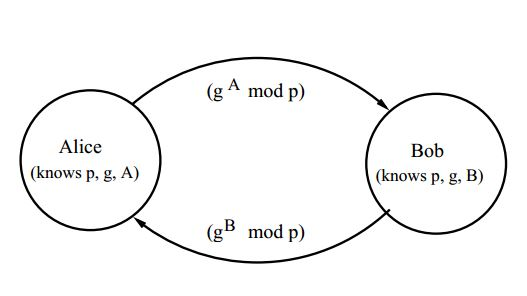
\includegraphics[width=0.7\linewidth]{Images/OR/dh.jpg}
  \caption{Illustration de l'algorithme Diffie-Hellman. \cite[Diffie-Hellman Algorithm.]{spider_diffie-hellman_2024}.}
  \label{fig:dh}
\end{figure}

La motivation principale de l'utilisation de \acrshort{dh} réside dans sa capacité à fournir un secret partagé qui peut ensuite être utilisé pour un chiffrement symétrique robuste, sans que la clé elle-même ne doive être transmise sur le réseau, offrant ainsi une sécurité contre les interceptions.
DH offre également le secret parfait vers l'avant: la compromission des clés privées n'entraîne pas celle des clés de sessions déjà établies.

% Le protocole Diffie-Hellman permet à deux parties de générer une clé secrète partagée sans la transmettre explicitement, en utilisant les étapes suivantes :

% \begin{enumerate}
  %   \item \textbf{Accord sur les paramètres communs :}
  %   Les deux parties s'accordent sur un nombre premier \( p \) et une base \( g \), qui sont publiques.
  
  %   \item \textbf{Génération des clés :}
  %   \begin{itemize}
  %     \item Alice choisit un nombre secret \( a \) et calcule \( A = g^a \mod p \).
  %     \item Bob choisit un nombre secret \( b \) et calcule \( B = g^b \mod p \).
  %     \item Ils échangent \( A \) et \( B \) respectivement.
  %   \end{itemize}
  
  %   \item \textbf{Génération de la clé partagée :}
  %   \begin{itemize}
  %     \item Alice reçoit \( B \) et calcule \( K = B^a \mod p \).
  %     \item Bob reçoit \( A \) et calcule \( K = A^b \mod p \).
  %   \end{itemize}
  % \end{enumerate}
  
  % Cette méthode assure que même si un attaquant peut écouter les échanges de \( A \) et \( B \), il ne peut pas calculer la clé partagée \( K \) sans résoudre le problème difficile du logarithme discret.


\subsubsection{TLS}\label{subsubsec:tls}

\acrfull{tls}, permet d'établir et de sécuriser les communications entre les relais en se basant sur une poignée de mains Diffie-Helman et une méthode de chiffrement (symétrique).

Le protocole \acrshort{tls} utilise donc une combinaison de cryptographie asymétrique pour l'échange de clés et l'authentification ainsi que de cryptographie symétrique pour le chiffrement des données.


\newpage
\section{Fonctionnement}\label{sec:works}

\acrshort{tor} est un réseau de serveurs, appelés nœuds ou relais, permettant aux utilisateurs d'accéder à Internet de manière anonyme.
Son fonctionnement est basé sur le principe de la transmission de données en couches chiffrées, d'où son nom qui fait référence à l'oignon ainsi qu'à ses couches. 
Cette section détaillera les étapes clés du processus permettant l'utilisation de \acrshort{tor} de l'"\nameref{subsec:initialisation}" à l' "\nameref{subsec:utilisation}" en passant par la "\nameref{subsec:construction}".

\subsection{Initialisation}\label{subsec:initialisation}

L'utilisateur initie la connexion avec le premier noeud.
\begin{enumerate}
  \item \textbf{Démarrage du Proxy Oignon (\acrshort{op}):} Il exécute d'un proxy oignon (\acrshort{op} \textit{Onion Proxy}) qui sert d'interface entre l'application utilisateur et le réseau \acrshort{tor}. 
  \item \textbf{Récupération des répertoires:} L'\acrshort{op} récupère la liste des  \acrshort{or}  actifs depuis les serveurs d'annuaires ainsi que les adresses, clés publiques et politiques de sorties.
  Ces informations signées permettent de vérifier leur authenticité.
  \item \textbf{Sélection des noeuds:}
  Les n\oe uds du circuit sont sélectionnés sur base de critères géographiques et liés aux politiques de sortie. De cette manière, l'anonymat ainsi que la compatibilité avec les besoins utilisateurs sont garantis.
  \item \textbf{Initialisation TLS:} L'\acrshort{op} établit une connexion \acrshort{tls} avec le gardien d'entrée (\textit{entry node}) afin de garantir la confidentialité et l'intégrité des communications initiales.
  Ce nœud connaît l'origine de la connexion mais ne connaît pas la destination finale des données.
\end{enumerate}

\subsection{Construction}\label{subsec:construction}

\acrshort{tor} crée un circuit chiffré à travers le réseau. 
\begin{enumerate}
  \item \textbf{Négociation Clé \acrlong{dh}:} Pour chaque  \acrshort{or}  sur le circuit, l'\acrshort{op} envoie une cellule "CREATE" contenant la première moitié d'un échange de clés \acrshort{dh}, chiffrée avec la clé publique de l' \acrshort{or}  (clé d'oignon). 
  Ce processus établit une clé de session symétrique partagée qui garantit que seul l' \acrshort{or}  peut déchiffrer et ainsi répondre à la requête.
  \item  \textbf{Extension du circuit:} L'\acrshort{op} envoie des cellules "RELAY EXTEND" à travers le circuit existant vers les autres  \acrshort{or}  pour négocier les nouvelles clés de session symétriques via \acrshort{dh}.
  Chaque  \acrshort{or}  ajoute sa propre couche de chiffrement afin de s'assurer que seuls les noeuds suivants puisse lire les instructions pour l'extension du circuit.
  \item \textbf{Vérification du circuit:} Le chiffrement itératif à chaque étape du circuit assure que chaque  \acrshort{or}  ne puisse accéder qu'aux informations de son prédécesseur et successeur direct.
\end{enumerate}

\subsection{Utilisation}\label{subsec:utilisation}

Les données passent ensuite par plusieurs nœuds intermédiaires (\textit{middle nodes}), où chaque nœud ne connaît que le nœud précédent et le suivant, mais jamais l'ensemble du circuit, comme expliqué dans.
\begin{enumerate}
  \item \textbf{Chiffrement en Couches :} Les données sont encapsulées dans des couches de chiffrement, une pour chaque nœud que le paquet de données traversera.
  \item \textbf{Déchiffrement Progressif :} À chaque étape du circuit, un nœud enlève une couche de chiffrement pour découvrir à quel nœud envoyer le paquet suivant.
  \item \textbf{Destination Finale :} 
  Lorsque les données atteignent le nœud de sortie (\textit{exit node}), la dernière couche de chiffrement est retirée et les données sont envoyées à leur destination finale.
\end{enumerate}

Grâce à ce mécanisme, l'adresse IP de l'utilisateur est masquée, et les données transmises sont rendues indéchiffrables pour les observateurs extérieurs.
Cela assure l'anonymat de l'utilisateur et la confidentialité des informations échangées.


% \subsection{Rôles}

% L'anonymisation implique différents rôles pour les noeuds selectionnés pour créer le circuit.


% \subsubsection{Sélection des Relais}
% Les relais sont choisis selon des critères stricts, visant à optimiser la performance et la sécurité. 
% La sélection tient compte de la bande passante, de la stabilité et de la réputation des relais, minimisant le risque d'attaques malveillantes.


% \subsection{Workflow}

% \begin{figure}[h!]
%   \centering
%   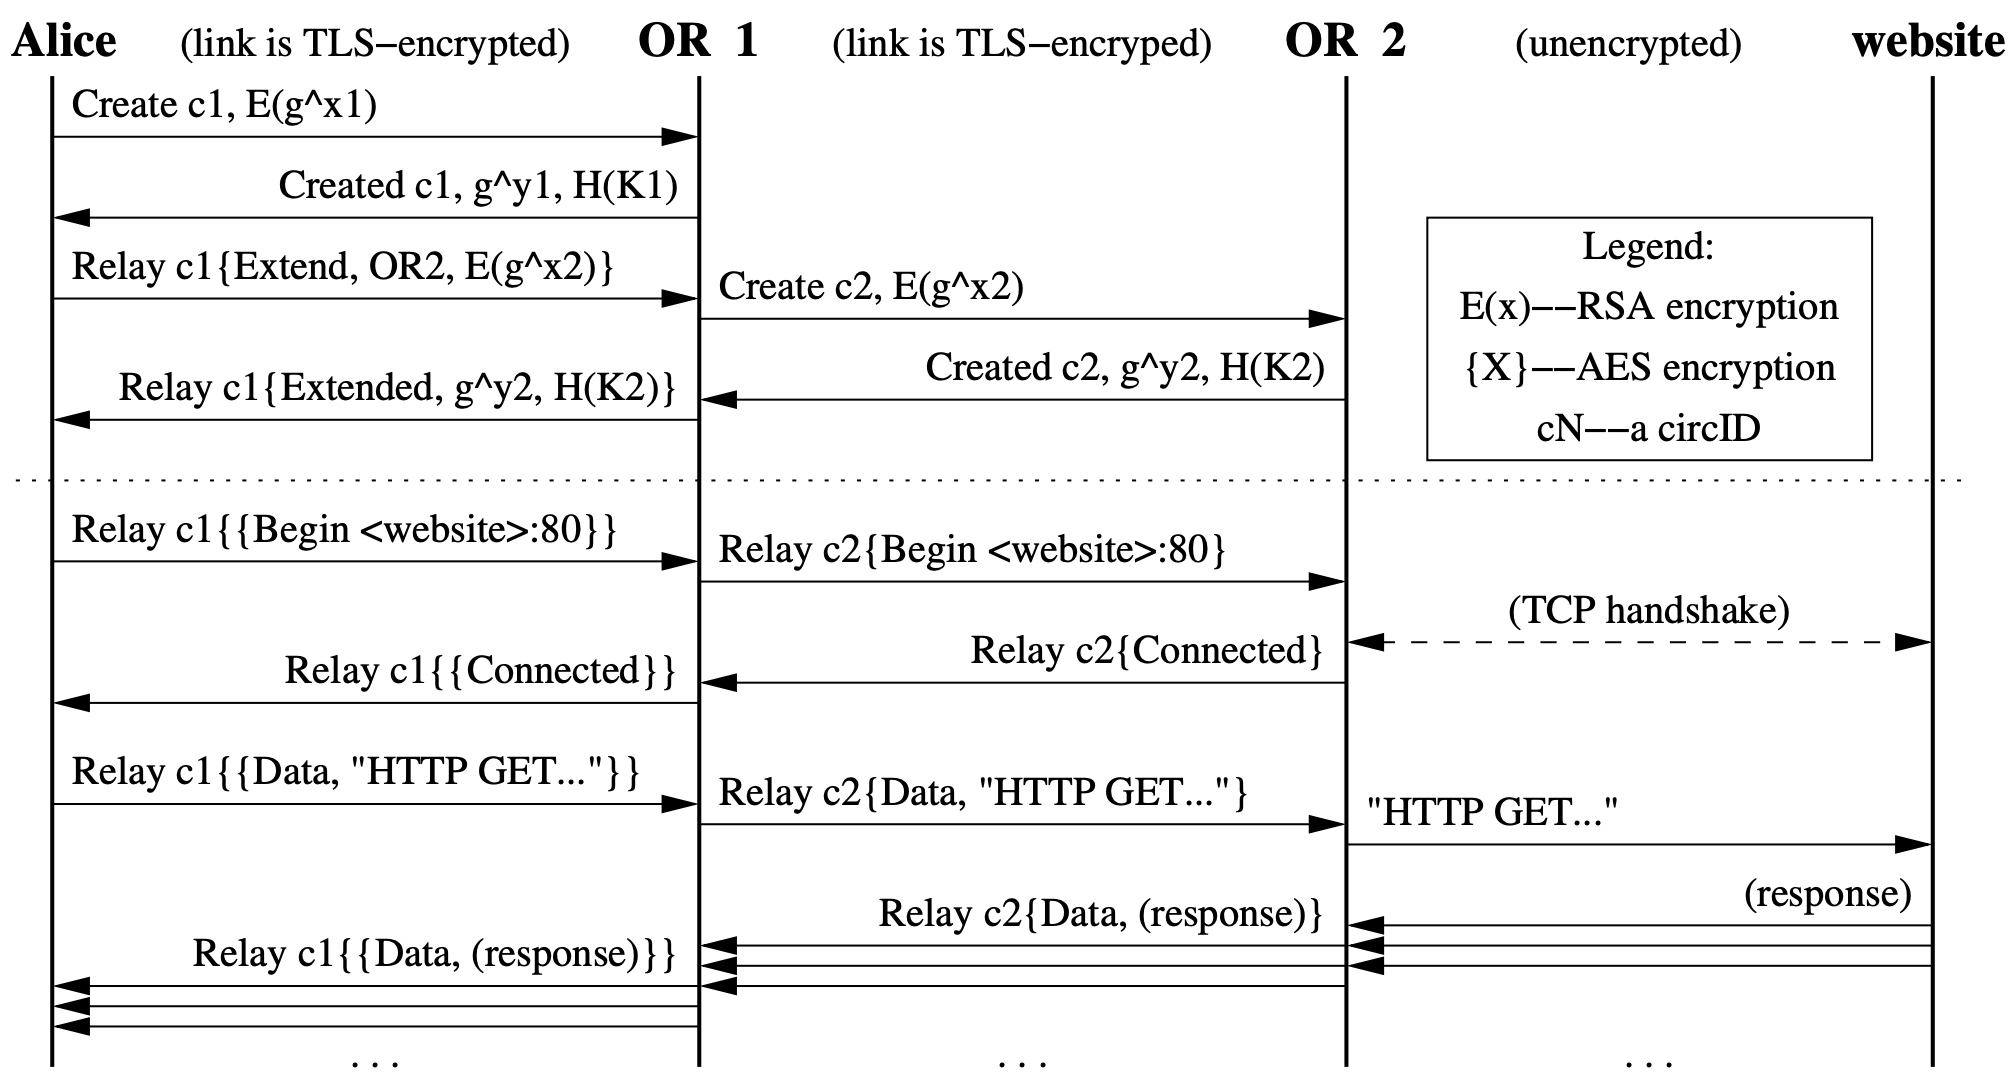
\includegraphics[width=\linewidth]{Images/Diagrams/flow.png}
%   \caption{Circuit à deux Routeurs Onions permettant à Alice de joindre un site web.\cite[Tor: The Second-Generation Onion Router]{dingledine_tor_2004}}
%   \label{fig:flowdiagram}
% \end{figure}

% \subsection{Services cachés}


% \newpage
% \section{Menaces}\label{sec:ad}

Comme décrit tout au long de ce rapport, \acrshort{tor} assure l'anonymat de ses client, la non-vulnérabilité des données qu'ils transmettent ainsi que l'intraçabilité de leurs communications de bout en bout. 
La présente section s'attardera sur les différents types d'attaques recensées dans l'article ainsi que les axes de défenses mis en place dans \acrshort{tor}.
L'anonymat sera abordé au point \ref{subsubsec:passive} "\nameref{subsubsec:passive}", les aspects cryptographiques au point \ref{subsubsec:active} "\nameref{subsubsec:active}".
Les servrus de répertoires au point \ref{subsubsec:annuaire} "\nameref{subsubsec:annuaire}" et les point de rendez-vous au \ref{subsubsec:rdv} "\nameref{subsubsec:rdv}".

\subsection{Passive}\label{subsubsec:passive}

Les attaques passives concernent uniquement l'établissement de profils sur base d'analyses permettant ainsi de compromettre l'anonymat. 
Le tableau \ref{tab:ad-passive} "\nameref{tab:ad-passive}" ci-dessous présente les différents types d'attaques passives recensées dans l'article et y associe un axe de défense.
\begin{table}[htpb]
    \centering
    \begin{tabularx}{\textwidth}{
        >{\raggedright\arraybackslash}X
        % p{4.5cm}
        >{\raggedright\arraybackslash}X}
    \toprule
    \rowcolor[HTML]{EFEFEF}
    \textbf{Menace}                          & \textbf{Solution} \\ 
    \midrule
    Observation des profils de trafic         & Le multiplexage de traffics sur un même circuit empêche l'analyse précise de profils de trafics. \\
    \midrule
    Observation du contenu utilisateur       & Si la destination est un noeud hostile, l'usage de \gls{privoxy}\footnote{Un privoxy est un proxy logiciel conçu spécialement pour \acrshort{tor} qui nettoye les protocoles d'application.} permet de conserver l'anonymat du client. \\
    \midrule
    Distinguabilité des options               & En permettant aux utilisateurs de confugurer leurs profils, cela compromet leur anonymat. \\
    \midrule
    Corrélation temporelle de bout en bout   & Masquer la communication entre le \acrshort{op} et le premier \acrshort{or} via un \acrshort{op} sur le \acrshort{or}. Cela contraint à séparer le traffic en provenance du trafic traversant. \\
    \midrule
    Corrélation de taille de bout en bout    & Rembourage\footnote{nombre différent de paquets autorisés} ou topologie du tuyau fuyant\footnote{Le tuyau fuyant (leaky pipe) est une topologie de circuit utilisée dans le réseau Tor pour améliorer l'anonymat des utilisateurs. Dans cette configuration, le trafic peut être dirigé pour sortir du circuit à des nœuds intermédiaires plutôt qu'à la fin du circuit. }. \\
    \midrule
    Empreintes digitales de site Web         & Multiplexage des flux, modification de la taille des cellules et rembourages. \\
    \bottomrule
    \end{tabularx}
    \caption{Menaces et défenses dans \acrshort{tor} : attaques passives}
    \label{tab:ad-passive}
\end{table}

\newpage
\subsection{Active}\label{subsubsec:active}

Les attaqques actives concernent uniquement la compromission des techniques de chiffrement via divers procédés. 
Le tableau \ref{tab:ad-active} "\nameref{tab:ad-active}" ci-dessous présente les différents types d'attaques actives recencées dans l'article et y associe un axe de défense.
\begin{table}[htpb]
    \centering
    \begin{tabularx}{\textwidth}{
        >{\raggedright\arraybackslash}p{4.5cm}
        >{\raggedright\arraybackslash}X}
    \toprule
    \rowcolor[HTML]{EFEFEF}
    \textbf{Menace}                                         & \textbf{Solution} \\
    \midrule
    Compromission des clés                                  & La rotation periodique permet de contrer la compromission des clés de sessions \acrshort{tls} car même si l'attaquant peut observer les cellules relayées sur chacun des circuits de cette connexion, sans la clé oignon, il ne peut déchiffrer le contenu. \\ 
    \midrule
    Compromission itérative                                 & Le secret parfait vers l'avant (\textit{i.e.} Perfect Forward Secrecy) empêche de remonter un circuit même si un attaque a lieu d'un \acrshort{or} intermédiaire jusqu'au dernier. \\ 
    \midrule
    Exploitation d'un serveur web                           & \acrshort{tor} dépend de \gls{privoxy} pour empêcher un serveur web d'identifier des profils temporels des utilisateurs qui s'y connectent d'adapter ses réponses. \\
    \midrule
    Exploitation d'un proxy onion                           & À un client ne peut correspondre qu'un \acrshort{op} local. Cependant, compromettre un proxy onion compromet toutes ses connexions. \\ 
    \midrule
    Attaque DoS sur des nœuds non observables               & La mise en place de stratégies permettant au réseau de garder le contrôle sur les ressources matérielles utilisables permet de contrer les attaques de type Déni de service (\textit{i.e.} \acrfull{dos}). \\
    \midrule
    Exploitation d'un \acrshort{or} hostile                 & Un nœud hostile doit etre immediatement adjacent aux deux extremites pour compromettre l'anonymat d'un circuit. Si un adversaire contrôle plus d'un \acrshort{or}, il ne peut compromettre plus qu'une partie du trafic. \\ 
    \midrule
    Introduction de timing dans les messages                & Cela représente une version plus forte des attaques de timing passives déjà discutées. \\ 
    \midrule
    Attaques par marquage                                   & Les contrôles d'intégrité\footnote{Initialisation d'un digest SHA-1} sur les cellules empêchent un n\oe ud hostile de marquer une cellule en la modifiant. \\ 
    \midrule
    Remplacement de contenus de protocoles non authentifiés & La préférence des clients pour des protocoles authentifiés de bout en bout permet d'empêcher un nœud de sortie hostile de se faire passer pour le serveur cible. \\
    \midrule
    Attaques par rejeu                                      & Le protocole d'échnage de clés \acrshort{dh} permet de renégocier de nouvelles clés de session et ainsi contrer les attaques par replay. \\ 
    \midrule
    Attaques de diffamation                                 & Les politiques de sorties réduisent l'impact des attaques par diffamation. \\ 
    \midrule
    Distribution de code hostile                            & Des clés publiques de version officielles du code de \acrshort{tor} permettent de vérifier son authenticité avant de l'exécuter. \\ 
    \bottomrule
    \end{tabularx}
    \caption{Menaces et défenses dans \acrshort{tor} : attaques actives}
    \label{tab:ad-active}
\end{table}


\newpage
\subsection{Annuaire}\label{subsubsec:annuaire}
Les serveurs d'annuaires sont un coposante essentielle de tout réseau \acrshort{tor}.
% Le Tableau \ref{tab:structure-annuaire} "\nameref{tab:structure-annuaire}" ci-dessous reprend la structure ainsi que le contenu typique d'un annuaire.
% \begin{table}[htpb]
\centering
\begin{tabularx}{\textwidth}{
    >{\raggedright\arraybackslash}p{4cm}
    >{\raggedright\arraybackslash}p{3cm}
    >{\raggedright\arraybackslash}X}
\toprule
\textbf{Catégorie} & \textbf{Elément} & \textbf{Description} \\
\midrule
\textbf{Liste des Routeurs d'Oignons} & 
   \textbf{Identifiants} & Chaque routeur a une clé publique unique utilisée pour l'identifier. \\
   & \textbf{Adresses IP et Ports} & Les adresses réseau et les ports sur lesquels les routeurs écoutent. \\
   & \textbf{Politiques de Sortie} & Les types de trafic que les routeurs acceptent ou rejettent (par exemple, blocage de certains ports). \\
\midrule
\textbf{État des Routeurs} &
    \textbf{Disponibilité} & Indique si un routeur est actuellement en ligne et accessible. \\
    & \textbf{Capacités} & Bande passante disponible, latence, et autres métriques de performance.\\
    & \textbf{Charges de Travail} & Informations sur la charge actuelle et la capacité du routeur à gérer plus de trafic. \\
 & \\
\midrule
\textbf{Clés Cryptographiques} &
    \textbf{Clés d'Identité} & Clés publiques utilisées pour vérifier l'identité du routeur. \\
    & \textbf{Certificats} & Signatures numériques qui certifient l'authenticité des clés et des informations publiées. \\
 & \\
\midrule
\textbf{Descripteurs de Serveurs} &
    \textbf{Descriptions Signées} & Déclarations signées par les routeurs eux-mêmes, détaillant leur état et leurs capacités. \\
    & \textbf{Horodatages} & Indiquent le moment où les informations ont été mises à jour pour assurer leur fraîcheur. \\
 & \\
\midrule
\textbf{Informations de Réseau} &
    \textbf{Topologie} & Vue d'ensemble de la disposition et des connexions entre les routeurs dans le réseau. \\
    & \textbf{Consensus} & Ensemble de données consolidées approuvé par plusieurs serveurs d'annuaire pour garantir la cohérence et la fiabilité des informations. \\
 & \\
\bottomrule
\end{tabularx}
\caption{Structure et contenu d'un annuaire.}
\label{tab:structure-annuaire}
\end{table}

Les attaques contre les serveurs d'annuaires ciblent celles dont l'objectif est la compromission d'une partie des circuits créés.
Le tableau \ref{tab:ad-ds} "\nameref{tab:ad-rdvp}" ci-dessous présente les différents types d'attaques contre les serveurs d'annuaires et y associe un axe de défense.
\begin{table}[htpb]
    \centering
    \begin{tabularx}{\textwidth}{
        >{\raggedright\arraybackslash}p{4.5cm}
        >{\raggedright\arraybackslash}X}
    \toprule
    \rowcolor[HTML]{EFEFEF}
    \textbf{Menace}                                                         & \textbf{Solution} \\ 
    \midrule
    Destruction des serveurs d'annuaires                                    & Tant que la moitié des serveurs d'annuaires sont en activité, ils continuent de fournir un annuaire valide. \\
    \midrule
    Subversion d'un serveur d'annuaire                                      & N'a qu'une influence partielle et minime sur la composition de l'annuaire final. \\
    \midrule
    Subversion de la majorité des serveurs d'annuaire                       & Les opérateurs de serveurs d'annuaires doivent être indépendants et résistants. \\
    \midrule
    Encouragement à la dissension entre serveurs d'annuaire                 & Aucune solution n'est proposée pour empecher de diviser les opérateurs et ainsi leurs utilisateurs. \\
    \midrule
    Tromper les serveurs d'annuaire pour lister un \acrshort{or} hostile    & Les opérateurs de serveurs de annuaire sont capables de filtrer la plupart des \acrshort{or}s hostiles. \\
    \midrule
    Convaincre les annuaires qu'un \acrshort{or} défaillant fonctionne      & Les serveurs d'annuaires doivent impérativement tester les \acrshort{or} de manière appropriée pour empêcher qu'un \acrshort{or} ne puisse accepter une connexion \acrshort{tls} en ignorant les cellules et ainsi passer les barrières de sécurité de \acrshort{tor}. \\
    \bottomrule
    \end{tabularx}
    \caption{Menaces et défenses dans \acrshort{tor} : serveurs d'annuaires}
    \label{tab:ad-ds}
\end{table}


\subsection{Points de rendez-vous}\label{subsubsec:rdv}

Les attaques contre les points de rendez-vous.
Le tableau \ref{tab:ad-rdvp} "\nameref{tab:ad-rdvp}" ci-dessous recence les différent types d'attaques contre les points de rendez-vous et y associe un axe de défense.
\begin{table}[htpb]
    \centering
    \begin{tabularx}{\textwidth}{
        >{\raggedright\arraybackslash}p{4.5cm}
        >{\raggedright\arraybackslash}X}
            \toprule
            \rowcolor[HTML]{EFEFEF}
            \textbf{Menace}                         & \textbf{Solution} \\
            \midrule
            Multiples demandes d'introduction       & Les points de rendez-vous peuvent bloquer les requêtes qui ne contiennent pas de jetons d'autorisation, de restreindre le nombre de requêtes recevables ou d'exiger une certaine quantité de calcul pour chaque requête reçue. \\
            \midrule
            Attaquer un point d'introduction        & Désactiver les points de rendez-vous mais ils sont liés à des clés publiques.  \\
            \midrule
            Compromission d'un point d'introduction & Un point de rendez-vous compromis peut inonder le trafic ou empêcher de nouvelles demandes.  \\
            \midrule
            Compromission d'un point de rendez-vous & Trafic chiffré par une clé de session. \\
            \bottomrule
    \end{tabularx}
    \caption{Menaces et défenses dans \acrshort{tor} : points de rendez-vous}
    \label{tab:ad-rdvp}
\end{table}


\newpage
\section{V3 Onion Services}\label{sec:v3}

Depuis 2021, \acrshort{tor} a abandonné la V2 des services oignons pour migrer vers la V3 \cite[A Comprehensive and Long-term Evaluation of \acrshort{tor} V3 Onion Services]{wang_comprehensive_2023} \cite[On the state of V3 onion services]{hoeller_state_2021}.

La principale différence entre les deux générations réside dans la complexité des clés: là où la v2 utilisait des adresses de 16 caractères dérivées d'une clé \acrshort{rsa} de 1024 bits, la v3 utilise quant à elle des adresses de 56 caractères dérivées d'une clé ED25519.
Ce qui contribue à renforcer leur sécurité.

De plus, les communications se voient également renforcées par l'utilisation de clés éphémères pour chaque session.

% Le tableau ci-dessous reprend les différences entre la V2 et la V3 
% \begin{table}[h!]
    \centering
    \begin{tabularx}{\textwidth}{
        >{\raggedright\arraybackslash}p{4cm}
        >{\raggedright\arraybackslash}X
        >{\raggedright\arraybackslash}X}
    \toprule
    \rowcolor[HTML]{EFEFEF}
    \textbf{Génération}             & \textbf{V2}                       & \textbf{V3} \\ 
    \midrule
    \textbf{Identification}         & Adresse .onion                    & Clé publique aveuglée (bpk) \\
    \textbf{Fuites d'information}   & Descripteurs non chiffrés         & Descripteurs chiffrés \\
    \textbf{Collecte d'adresses}    & Possible par les relais HSDir     & Prévention par dérivation de clé \\
    \textbf{Influence sur HSDir}    & Choix d'empreinte manipulable     & Valeur aléatoire partagée réduit l'influence \\
    \textbf{Prévisibilité}          & Position prédictible dans HSDir   & Positions imprévisibles grâce à la valeur aléatoire \\
    \textbf{Attaque par ombrage}    & Réalisable par manipulation       & Mitigée par des changements de conception \\
    \bottomrule
    \end{tabularx}
    \caption{Comparaison des services onion V2 et V3 et solutions V3 aux menaces V2}
    \label{table:1}
\end{table}

\newpage
\section{Conclusion}\label{sec:conclusion}



\newpage
\appendix
% \section{Différence entre \acrshort{tls} et le chiffrement par clé}
% \begin{table}[htbp]
    \centering
    \begin{tabularx}{\textwidth}{
        >{\raggedright\arraybackslash}p{2cm} 
        >{\raggedright\arraybackslash}X 
        >{\raggedright\arraybackslash}X}
        \toprule
        \rowcolor[HTML]{EFEFEF}
        \textbf{}           & \textbf{TLS}                                                                      & \textbf{Chiffrement par clé} \\
        \midrule
        Nature              & Protocole de sécurité pour les communications réseau                              & Méthode pour chiffrer/déchiffrer des données \\
        \midrule
        Utilisation de clés & Utilise à la fois des clés symétriques et asymétriques                            & Peut utiliser des clés symétriques ou asymétriques \\
        \midrule
        Objectif principal  & Sécuriser des sessions ou connexions entières                                     & Sécuriser des données ou messages spécifiques \\
        \midrule
        Mise en œuvre       & Négocie les paramètres de chiffrement avant le transfert de données               & Appliqué aux données elles-mêmes, indépendamment du canal \\
        \midrule
        Applications        & Sécurisation du web (HTTPS), courrier électronique, messagerie instantanée, etc.  & Chiffrement de fichiers, communication sécurisée, authentification, signature numérique \\
        \bottomrule
    \end{tabularx}
    \caption{Comparaison entre \acrshort{tls} et le chiffrement par clé}
    \label{tab:TLSvsKeyEncryption}
\end{table}

% \section{Différents types d'attaques}
% \begin{longtable}{p{0.25\linewidth} p{0.7\linewidth}}
    \toprule
    \textbf{Attaque} & \textbf{Défense} \\
    \midrule
    Observation du trafic utilisateur & Le contenu à l'extrémité de l'utilisateur est crypté, bien que les connexions aux répondants puissent ne pas l'être. \\
    \addlinespace
    Corrélation de timing de bout en bout & \acrshort{tor} minimise mais ne cache pas complètement ces corrélations. \\
    \addlinespace
    Corrélation de la taille de bout en bout & La multiplexation des flux dans le même circuit limite cette corrélation à la granularité des cellules. \\
    \addlinespace
    Empreinte digitale de site web & Potentiellement effective contre Tor; des défenses supplémentaires pourraient inclure des stratégies de padding. \\
    \addlinespace
    Compromission de clés & La rotation périodique des clés limite la fenêtre d'opportunité pour ces attaques. \\
    \addlinespace
    Compromission d'un \acrshort{or} par itération & \acrshort{tor} protège contre ce scénario en éliminant rapidement les informations nécessaires pour compléter une telle attaque. \\
    \addlinespace
    Exécution d'un serveur de destination hostile & Les attaques de fin à fin deviennent plus faciles si l'adversaire peut induire les utilisateurs à se connecter à son serveur web. \\
    \addlinespace
    Exécution d'un \acrshort{or} hostile & Un \acrshort{or} isolé hostile peut créer des circuits à travers lui-même ou altérer des modèles de trafic. \\
    \addlinespace
    Introduire un timing dans les messages & \acrshort{tor} n'adresse pas directement ces attaques, mais elles ne sont qu'une version plus forte des attaques passives de timing. \\
    \addlinespace
    Attaques de tag & Les vérifications d'intégrité sur les cellules empêchent cette attaque. \\
    \addlinespace
    Remplacement de contenus de protocoles non authentifiés & Un nœud de sortie hostile peut usurper le serveur cible pour des protocoles non authentifiés. \\
    \addlinespace
    Attaques de replay & Non pertinentes pour Tor; la rediffusion d'un côté de la poignée de main entraîne une clé de session différente. \\
    \addlinespace
    Attaques contre les points de rendez-vous & Bob peut limiter la réception de requêtes via des tokens d'autorisation, et les points d'introduction peuvent être secrètement annoncés. \\
    \addlinespace
    Attaques contre les serveurs de répertoire & Si un serveur de répertoire est compromis, il peut partiellement influencer le répertoire final, mais une majorité est nécessaire pour inclure des \acrshort{or} compromis. \\
    \bottomrule
    \end{longtable}

\section{Latence et anonymat}
Dans les sytèmes de communication en réseau, le niveau d'anonymat est toujours corrélé avec le niveau de latence de ce système.

L'anonymat d'un client sur un réseau informatique lui confère l'intraçabilité de son activité en ligne.
Dans le cadre de \acrshort{tor}, cela est réalisé via le routage du trafic à travers plusieurs n\oe uds ou \acrfull{or}: chaque n\oe ud n'ayant connaissance que de son prédécesseur ainsi que de son successeur.

La latence - somme des délais - dans un réseau informatique désigne le temps écoulé entre l'envoi d'un paquet de données depuis une source et sa réception par la destination.
Dans le cadre de \acrshort{tor}, son accroissement s'explique d'une part par la répartition géographique globale des \acrshort{or} (\textit{cfr,} \acrfull{pd}) et d'autre part par les délais de chiffrement, déchiffrement qui surviennent à chaque \acrshort{or} (\textit{cfr,} \acrfull{td}).

Cette latence est donc un compromis nécessaire pour obtenir un niveau élevé d'anonymat et de sécurité, car elle rend plus difficile pour un observateur de corréler le trafic entrant et sortant.


\section{Menaces}\label{sec:ad}

Comme décrit tout au long de ce rapport, \acrshort{tor} assure l'anonymat de ses client, la non-vulnérabilité des données qu'ils transmettent ainsi que l'intraçabilité de leurs communications de bout en bout. 
La présente section s'attardera sur les différents types d'attaques recensées dans l'article ainsi que les axes de défenses mis en place dans \acrshort{tor}.
L'anonymat sera abordé au point \ref{subsubsec:passive} "\nameref{subsubsec:passive}", les aspects cryptographiques au point \ref{subsubsec:active} "\nameref{subsubsec:active}".
Les servrus de répertoires au point \ref{subsubsec:annuaire} "\nameref{subsubsec:annuaire}" et les point de rendez-vous au \ref{subsubsec:rdv} "\nameref{subsubsec:rdv}".

\subsection{Passive}\label{subsubsec:passive}

Les attaques passives concernent uniquement l'établissement de profils sur base d'analyses permettant ainsi de compromettre l'anonymat. 
Le tableau \ref{tab:ad-passive} "\nameref{tab:ad-passive}" ci-dessous présente les différents types d'attaques passives recensées dans l'article et y associe un axe de défense.
\begin{table}[htpb]
    \centering
    \begin{tabularx}{\textwidth}{
        >{\raggedright\arraybackslash}X
        % p{4.5cm}
        >{\raggedright\arraybackslash}X}
    \toprule
    \rowcolor[HTML]{EFEFEF}
    \textbf{Menace}                          & \textbf{Solution} \\ 
    \midrule
    Observation des profils de trafic         & Le multiplexage de traffics sur un même circuit empêche l'analyse précise de profils de trafics. \\
    \midrule
    Observation du contenu utilisateur       & Si la destination est un noeud hostile, l'usage de \gls{privoxy}\footnote{Un privoxy est un proxy logiciel conçu spécialement pour \acrshort{tor} qui nettoye les protocoles d'application.} permet de conserver l'anonymat du client. \\
    \midrule
    Distinguabilité des options               & En permettant aux utilisateurs de confugurer leurs profils, cela compromet leur anonymat. \\
    \midrule
    Corrélation temporelle de bout en bout   & Masquer la communication entre le \acrshort{op} et le premier \acrshort{or} via un \acrshort{op} sur le \acrshort{or}. Cela contraint à séparer le traffic en provenance du trafic traversant. \\
    \midrule
    Corrélation de taille de bout en bout    & Rembourage\footnote{nombre différent de paquets autorisés} ou topologie du tuyau fuyant\footnote{Le tuyau fuyant (leaky pipe) est une topologie de circuit utilisée dans le réseau Tor pour améliorer l'anonymat des utilisateurs. Dans cette configuration, le trafic peut être dirigé pour sortir du circuit à des nœuds intermédiaires plutôt qu'à la fin du circuit. }. \\
    \midrule
    Empreintes digitales de site Web         & Multiplexage des flux, modification de la taille des cellules et rembourages. \\
    \bottomrule
    \end{tabularx}
    \caption{Menaces et défenses dans \acrshort{tor} : attaques passives}
    \label{tab:ad-passive}
\end{table}

\newpage
\subsection{Active}\label{subsubsec:active}

Les attaqques actives concernent uniquement la compromission des techniques de chiffrement via divers procédés. 
Le tableau \ref{tab:ad-active} "\nameref{tab:ad-active}" ci-dessous présente les différents types d'attaques actives recencées dans l'article et y associe un axe de défense.
\begin{table}[htpb]
    \centering
    \begin{tabularx}{\textwidth}{
        >{\raggedright\arraybackslash}p{4.5cm}
        >{\raggedright\arraybackslash}X}
    \toprule
    \rowcolor[HTML]{EFEFEF}
    \textbf{Menace}                                         & \textbf{Solution} \\
    \midrule
    Compromission des clés                                  & La rotation periodique permet de contrer la compromission des clés de sessions \acrshort{tls} car même si l'attaquant peut observer les cellules relayées sur chacun des circuits de cette connexion, sans la clé oignon, il ne peut déchiffrer le contenu. \\ 
    \midrule
    Compromission itérative                                 & Le secret parfait vers l'avant (\textit{i.e.} Perfect Forward Secrecy) empêche de remonter un circuit même si un attaque a lieu d'un \acrshort{or} intermédiaire jusqu'au dernier. \\ 
    \midrule
    Exploitation d'un serveur web                           & \acrshort{tor} dépend de \gls{privoxy} pour empêcher un serveur web d'identifier des profils temporels des utilisateurs qui s'y connectent d'adapter ses réponses. \\
    \midrule
    Exploitation d'un proxy onion                           & À un client ne peut correspondre qu'un \acrshort{op} local. Cependant, compromettre un proxy onion compromet toutes ses connexions. \\ 
    \midrule
    Attaque DoS sur des nœuds non observables               & La mise en place de stratégies permettant au réseau de garder le contrôle sur les ressources matérielles utilisables permet de contrer les attaques de type Déni de service (\textit{i.e.} \acrfull{dos}). \\
    \midrule
    Exploitation d'un \acrshort{or} hostile                 & Un nœud hostile doit etre immediatement adjacent aux deux extremites pour compromettre l'anonymat d'un circuit. Si un adversaire contrôle plus d'un \acrshort{or}, il ne peut compromettre plus qu'une partie du trafic. \\ 
    \midrule
    Introduction de timing dans les messages                & Cela représente une version plus forte des attaques de timing passives déjà discutées. \\ 
    \midrule
    Attaques par marquage                                   & Les contrôles d'intégrité\footnote{Initialisation d'un digest SHA-1} sur les cellules empêchent un n\oe ud hostile de marquer une cellule en la modifiant. \\ 
    \midrule
    Remplacement de contenus de protocoles non authentifiés & La préférence des clients pour des protocoles authentifiés de bout en bout permet d'empêcher un nœud de sortie hostile de se faire passer pour le serveur cible. \\
    \midrule
    Attaques par rejeu                                      & Le protocole d'échnage de clés \acrshort{dh} permet de renégocier de nouvelles clés de session et ainsi contrer les attaques par replay. \\ 
    \midrule
    Attaques de diffamation                                 & Les politiques de sorties réduisent l'impact des attaques par diffamation. \\ 
    \midrule
    Distribution de code hostile                            & Des clés publiques de version officielles du code de \acrshort{tor} permettent de vérifier son authenticité avant de l'exécuter. \\ 
    \bottomrule
    \end{tabularx}
    \caption{Menaces et défenses dans \acrshort{tor} : attaques actives}
    \label{tab:ad-active}
\end{table}


\newpage
\subsection{Annuaire}\label{subsubsec:annuaire}
Les serveurs d'annuaires sont un coposante essentielle de tout réseau \acrshort{tor}.
% Le Tableau \ref{tab:structure-annuaire} "\nameref{tab:structure-annuaire}" ci-dessous reprend la structure ainsi que le contenu typique d'un annuaire.
% \begin{table}[htpb]
\centering
\begin{tabularx}{\textwidth}{
    >{\raggedright\arraybackslash}p{4cm}
    >{\raggedright\arraybackslash}p{3cm}
    >{\raggedright\arraybackslash}X}
\toprule
\textbf{Catégorie} & \textbf{Elément} & \textbf{Description} \\
\midrule
\textbf{Liste des Routeurs d'Oignons} & 
   \textbf{Identifiants} & Chaque routeur a une clé publique unique utilisée pour l'identifier. \\
   & \textbf{Adresses IP et Ports} & Les adresses réseau et les ports sur lesquels les routeurs écoutent. \\
   & \textbf{Politiques de Sortie} & Les types de trafic que les routeurs acceptent ou rejettent (par exemple, blocage de certains ports). \\
\midrule
\textbf{État des Routeurs} &
    \textbf{Disponibilité} & Indique si un routeur est actuellement en ligne et accessible. \\
    & \textbf{Capacités} & Bande passante disponible, latence, et autres métriques de performance.\\
    & \textbf{Charges de Travail} & Informations sur la charge actuelle et la capacité du routeur à gérer plus de trafic. \\
 & \\
\midrule
\textbf{Clés Cryptographiques} &
    \textbf{Clés d'Identité} & Clés publiques utilisées pour vérifier l'identité du routeur. \\
    & \textbf{Certificats} & Signatures numériques qui certifient l'authenticité des clés et des informations publiées. \\
 & \\
\midrule
\textbf{Descripteurs de Serveurs} &
    \textbf{Descriptions Signées} & Déclarations signées par les routeurs eux-mêmes, détaillant leur état et leurs capacités. \\
    & \textbf{Horodatages} & Indiquent le moment où les informations ont été mises à jour pour assurer leur fraîcheur. \\
 & \\
\midrule
\textbf{Informations de Réseau} &
    \textbf{Topologie} & Vue d'ensemble de la disposition et des connexions entre les routeurs dans le réseau. \\
    & \textbf{Consensus} & Ensemble de données consolidées approuvé par plusieurs serveurs d'annuaire pour garantir la cohérence et la fiabilité des informations. \\
 & \\
\bottomrule
\end{tabularx}
\caption{Structure et contenu d'un annuaire.}
\label{tab:structure-annuaire}
\end{table}

Les attaques contre les serveurs d'annuaires ciblent celles dont l'objectif est la compromission d'une partie des circuits créés.
Le tableau \ref{tab:ad-ds} "\nameref{tab:ad-rdvp}" ci-dessous présente les différents types d'attaques contre les serveurs d'annuaires et y associe un axe de défense.
\begin{table}[htpb]
    \centering
    \begin{tabularx}{\textwidth}{
        >{\raggedright\arraybackslash}p{4.5cm}
        >{\raggedright\arraybackslash}X}
    \toprule
    \rowcolor[HTML]{EFEFEF}
    \textbf{Menace}                                                         & \textbf{Solution} \\ 
    \midrule
    Destruction des serveurs d'annuaires                                    & Tant que la moitié des serveurs d'annuaires sont en activité, ils continuent de fournir un annuaire valide. \\
    \midrule
    Subversion d'un serveur d'annuaire                                      & N'a qu'une influence partielle et minime sur la composition de l'annuaire final. \\
    \midrule
    Subversion de la majorité des serveurs d'annuaire                       & Les opérateurs de serveurs d'annuaires doivent être indépendants et résistants. \\
    \midrule
    Encouragement à la dissension entre serveurs d'annuaire                 & Aucune solution n'est proposée pour empecher de diviser les opérateurs et ainsi leurs utilisateurs. \\
    \midrule
    Tromper les serveurs d'annuaire pour lister un \acrshort{or} hostile    & Les opérateurs de serveurs de annuaire sont capables de filtrer la plupart des \acrshort{or}s hostiles. \\
    \midrule
    Convaincre les annuaires qu'un \acrshort{or} défaillant fonctionne      & Les serveurs d'annuaires doivent impérativement tester les \acrshort{or} de manière appropriée pour empêcher qu'un \acrshort{or} ne puisse accepter une connexion \acrshort{tls} en ignorant les cellules et ainsi passer les barrières de sécurité de \acrshort{tor}. \\
    \bottomrule
    \end{tabularx}
    \caption{Menaces et défenses dans \acrshort{tor} : serveurs d'annuaires}
    \label{tab:ad-ds}
\end{table}


\subsection{Points de rendez-vous}\label{subsubsec:rdv}

Les attaques contre les points de rendez-vous.
Le tableau \ref{tab:ad-rdvp} "\nameref{tab:ad-rdvp}" ci-dessous recence les différent types d'attaques contre les points de rendez-vous et y associe un axe de défense.
\begin{table}[htpb]
    \centering
    \begin{tabularx}{\textwidth}{
        >{\raggedright\arraybackslash}p{4.5cm}
        >{\raggedright\arraybackslash}X}
            \toprule
            \rowcolor[HTML]{EFEFEF}
            \textbf{Menace}                         & \textbf{Solution} \\
            \midrule
            Multiples demandes d'introduction       & Les points de rendez-vous peuvent bloquer les requêtes qui ne contiennent pas de jetons d'autorisation, de restreindre le nombre de requêtes recevables ou d'exiger une certaine quantité de calcul pour chaque requête reçue. \\
            \midrule
            Attaquer un point d'introduction        & Désactiver les points de rendez-vous mais ils sont liés à des clés publiques.  \\
            \midrule
            Compromission d'un point d'introduction & Un point de rendez-vous compromis peut inonder le trafic ou empêcher de nouvelles demandes.  \\
            \midrule
            Compromission d'un point de rendez-vous & Trafic chiffré par une clé de session. \\
            \bottomrule
    \end{tabularx}
    \caption{Menaces et défenses dans \acrshort{tor} : points de rendez-vous}
    \label{tab:ad-rdvp}
\end{table}


\newpage
\renewcommand{\listfigurename}{Figures}
\listoffigures
\addcontentsline{toc}{section}{\listfigurename}

\newpage
\renewcommand{\listtablename}{Tableaux}
\listoftables
\addcontentsline{toc}{section}{\listtablename}

\newpage
\renewcommand{\listalgorithmname}{Algorithmes}
\listofalgorithms
\addcontentsline{toc}{section}{\listalgorithmname}

\newpage
% \renewcommand{\printglossary}{Glossaire}
\printglossary[title=Glossaire,toctitle=Glossaire]
% \printglossary[type=\acronymtype]
% \printglossaries

\newpage
\printbibliography[title=Références]

\end{document}